\documentclass[twoside]{book}

% Packages required by doxygen
\usepackage{calc}
\usepackage{doxygen}
\usepackage{graphicx}
\usepackage[utf8]{inputenc}
\usepackage{makeidx}
\usepackage{multicol}
\usepackage{multirow}
\usepackage{textcomp}
\usepackage[table]{xcolor}

% Font selection
\usepackage[T1]{fontenc}
\usepackage{mathptmx}
\usepackage[scaled=.90]{helvet}
\usepackage{courier}
\usepackage{amssymb}
\usepackage{sectsty}
\renewcommand{\familydefault}{\sfdefault}
\allsectionsfont{%
  \fontseries{bc}\selectfont%
  \color{darkgray}%
}
\renewcommand{\DoxyLabelFont}{%
  \fontseries{bc}\selectfont%
  \color{darkgray}%
}

% Page & text layout
\usepackage{geometry}
\geometry{%
  a4paper,%
  top=2.5cm,%
  bottom=2.5cm,%
  left=2.5cm,%
  right=2.5cm%
}
\tolerance=750
\hfuzz=15pt
\hbadness=750
\setlength{\emergencystretch}{15pt}
\setlength{\parindent}{0cm}
\setlength{\parskip}{0.2cm}
\makeatletter
\renewcommand{\paragraph}{%
  \@startsection{paragraph}{4}{0ex}{-1.0ex}{1.0ex}{%
    \normalfont\normalsize\bfseries\SS@parafont%
  }%
}
\renewcommand{\subparagraph}{%
  \@startsection{subparagraph}{5}{0ex}{-1.0ex}{1.0ex}{%
    \normalfont\normalsize\bfseries\SS@subparafont%
  }%
}
\makeatother

% Headers & footers
\usepackage{fancyhdr}
\pagestyle{fancyplain}
\fancyhead[LE]{\fancyplain{}{\bfseries\thepage}}
\fancyhead[CE]{\fancyplain{}{}}
\fancyhead[RE]{\fancyplain{}{\bfseries\leftmark}}
\fancyhead[LO]{\fancyplain{}{\bfseries\rightmark}}
\fancyhead[CO]{\fancyplain{}{}}
\fancyhead[RO]{\fancyplain{}{\bfseries\thepage}}
\fancyfoot[LE]{\fancyplain{}{}}
\fancyfoot[CE]{\fancyplain{}{}}
\fancyfoot[RE]{\fancyplain{}{\bfseries\scriptsize Generated on Sun Feb 8 2015 23\-:09\-:36 for Doc Projet T\-L by Doxygen }}
\fancyfoot[LO]{\fancyplain{}{\bfseries\scriptsize Generated on Sun Feb 8 2015 23\-:09\-:36 for Doc Projet T\-L by Doxygen }}
\fancyfoot[CO]{\fancyplain{}{}}
\fancyfoot[RO]{\fancyplain{}{}}
\renewcommand{\footrulewidth}{0.4pt}
\renewcommand{\chaptermark}[1]{%
  \markboth{#1}{}%
}
\renewcommand{\sectionmark}[1]{%
  \markright{\thesection\ #1}%
}

% Indices & bibliography
\usepackage{natbib}
\usepackage[titles]{tocloft}
\setcounter{tocdepth}{3}
\setcounter{secnumdepth}{5}
\makeindex

% Hyperlinks (required, but should be loaded last)
\usepackage{ifpdf}
\ifpdf
  \usepackage[pdftex,pagebackref=true]{hyperref}
\else
  \usepackage[ps2pdf,pagebackref=true]{hyperref}
\fi
\hypersetup{%
  colorlinks=true,%
  linkcolor=blue,%
  citecolor=blue,%
  unicode%
}

% Custom commands
\newcommand{\clearemptydoublepage}{%
  \newpage{\pagestyle{empty}\cleardoublepage}%
}


%===== C O N T E N T S =====

\begin{document}

% Titlepage & ToC
\hypersetup{pageanchor=false}
\pagenumbering{roman}
\begin{titlepage}
\vspace*{7cm}
\begin{center}%
{\Large Doc Projet T\-L }\\
\vspace*{1cm}
{\large Generated by Doxygen 1.8.6}\\
\vspace*{0.5cm}
{\small Sun Feb 8 2015 23:09:36}\\
\end{center}
\end{titlepage}
\clearemptydoublepage
\tableofcontents
\clearemptydoublepage
\pagenumbering{arabic}
\hypersetup{pageanchor=true}

%--- Begin generated contents ---
\chapter{Documentation du logiciel Autoroute}
\label{index}\hypertarget{index}{}\hypertarget{index_intro_sec}{}\section{Introduction}\label{index_intro_sec}
En allant dans la section Classes, vous aurait accès à la documentation de l'ensemble des classes. A partir de là, vous pourrez trouvez de la doc concernant les attributs et méthodes des classes.

Dans cette page principale, nous verrons comment exécuter le logiciel Autoroute, prendre en main les sources, l'arborescence du projet ainsi que des définitions relatives à la théorie des langages et aux automates.\hypertarget{index_install_sec}{}\section{Installation du logiciel pour les utilisateurs}\label{index_install_sec}
\hypertarget{index_windows}{}\subsection{Windows \-:}\label{index_windows}
Installer qt5, graphviz puis le setup d'autoroute que vous trouverez dans le dossier exe.\hypertarget{index_linux}{}\subsection{Linux \-:}\label{index_linux}
Installer qt5 et graphviz. Lancer qt5 et ouvrez un projet, sélectionnez le fichier autoroute.\-pro dans le dossier automate-\/project. Cliquez ensuite sur la flèche verte (Run) en bas à gauche de la fenêtre.\hypertarget{index_dev_sec}{}\section{Pour les développeurs}\label{index_dev_sec}
\hypertarget{index_etape1}{}\subsection{Etape 1 \-: Prise en main des sources et execution}\label{index_etape1}
Ce logiciel est développé en C++, avec le framework Q\-T5. La manière la plus simple d'accéder aux sources, d'exécuter le programme et de modifier ce logiciel est la suivante \-:
\begin{DoxyItemize}
\item installer Q\-T
\item créer un dossier dans lequel vous mettrez les 3 dossiers (executable, doc et automate-\/project)
\item dans Q\-T, cliquez sur Open a project puis allez chercher le fichier automate-\/project/autoroute.\-pro
\item pour lancer le logiciel, cliquez simplement sur la flèche verte
\end{DoxyItemize}

Il vous faudra peut-\/être configurer dans l'onglet \char`\"{}\-Projects\char`\"{} l'exécution. Il suffit normalement de préciser le dossier automate/project et d'utiliser les paramètres par défaut.

N\-B \-: Vous aurez peut-\/être un problème de version si vous avez une version supérieure à Q\-T5. Il suffit en général de modifier le nom des bibliothèques. Si cela ne change pas, il vous reste plusieurs solutions \-:
\begin{DoxyItemize}
\item aller voir sur le net comment passer le projet de Q\-T5 à la version actuelle de Q\-T
\item résoudre les erreurs de compilation (aidez vous du debugger de Q\-T), c'est la solution conseillée.
\end{DoxyItemize}\hypertarget{index_etape2}{}\subsection{Etape 2 \-: Arborescence du projet}\label{index_etape2}
\begin{DoxyVerb}   - doc/ : vous trouverez ici deux dossiers (html et latex) correspondant à deux formats de la documentation. Il y aussi dans ce dossier les comptes rendus 2010 et 2015.
\end{DoxyVerb}
 Il est possible d'ouvrir ce fichier avec Doxygen et de générer la documentation du programme si vous voulez la modifier. Ce tutoriel est assez bien fait pour prendre en main doxygen \-: \href{http://franckh.developpez.com/tutoriels/outils/doxygen/}{\tt http\-://franckh.\-developpez.\-com/tutoriels/outils/doxygen/}

\begin{DoxyVerb}   - automate-project/ : les sources du programme.
\end{DoxyVerb}
 Mieux vaux ne pas y toucher au début, surtout si l'on ne connait pas Q\-T et modifier le code seulement via Q\-T. \begin{DoxyVerb}  - executable/ : tout les fichiers relatifs aux exécutables
\end{DoxyVerb}
\hypertarget{index_definitions}{}\section{Définitions}\label{index_definitions}
\hypertarget{index_minimisation}{}\subsection{Minimisation d'un automate}\label{index_minimisation}
La minimisation d'un automate fini déterministe est l'opération qui consiste à transformer un automate fini déterministe donné en un automate fini déterministe ayant le nombre minimal d'états et qui reconnaît le même langage rationnel.\hypertarget{index_standardisation}{}\subsection{Standardisation d'un automate}\label{index_standardisation}
Un automate fini est dit standard si aucune transition n'arrive sur son seul état initial.\hypertarget{index_produit}{}\subsection{Produit de deux automates}\label{index_produit}
On veut calculer un automate qui reconnaisse le langage L1$^\wedge$\-L2, c'est-\/à-\/dire le langage des mots qui sont reconnus à la fois par A1 et A2. On construit pour cela le produit de deux automates.\hypertarget{index_determinisation}{}\subsection{Déterminisation de deux automates}\label{index_determinisation}
En informatique, le déterminisme est le fait de ne pas avoir le choix entre plusieurs exécutions. Pour les automates finis, cela correspond à avoir, pour chaque état et pour une étiquette (de transition) donnée, au plus une seule transition portant cette étiquette et partant de cet état. 
\chapter{Hierarchical Index}
\section{Class Hierarchy}
This inheritance list is sorted roughly, but not completely, alphabetically\-:\begin{DoxyCompactList}
\item \contentsline{section}{Automate}{\pageref{class_automate}}{}
\item \contentsline{section}{etat}{\pageref{classetat}}{}
\item Q\-Main\-Window\begin{DoxyCompactList}
\item \contentsline{section}{Create\-Automate}{\pageref{class_create_automate}}{}
\item \contentsline{section}{Main\-Window}{\pageref{class_main_window}}{}
\end{DoxyCompactList}
\item Q\-Widget\begin{DoxyCompactList}
\item \contentsline{section}{choix\-Pointe}{\pageref{classchoix_pointe}}{}
\item \contentsline{section}{etat\-Left}{\pageref{classetat_left}}{}
\item \contentsline{section}{etat\-Right}{\pageref{classetat_right}}{}
\item \contentsline{section}{Transition}{\pageref{class_transition}}{}
\end{DoxyCompactList}
\end{DoxyCompactList}

\chapter{Class Index}
\section{Class List}
Here are the classes, structs, unions and interfaces with brief descriptions\-:\begin{DoxyCompactList}
\item\contentsline{section}{\hyperlink{class_automate}{Automate} }{\pageref{class_automate}}{}
\item\contentsline{section}{\hyperlink{classchoix_pointe}{choix\-Pointe} }{\pageref{classchoix_pointe}}{}
\item\contentsline{section}{\hyperlink{class_ui_1_1choix_pointe}{Ui\-::choix\-Pointe} }{\pageref{class_ui_1_1choix_pointe}}{}
\item\contentsline{section}{\hyperlink{class_ui_1_1_create_automate}{Ui\-::\-Create\-Automate} }{\pageref{class_ui_1_1_create_automate}}{}
\item\contentsline{section}{\hyperlink{class_create_automate}{Create\-Automate} }{\pageref{class_create_automate}}{}
\item\contentsline{section}{\hyperlink{classetat}{etat} }{\pageref{classetat}}{}
\item\contentsline{section}{\hyperlink{classetat_left}{etat\-Left} }{\pageref{classetat_left}}{}
\item\contentsline{section}{\hyperlink{class_ui_1_1etat_left}{Ui\-::etat\-Left} }{\pageref{class_ui_1_1etat_left}}{}
\item\contentsline{section}{\hyperlink{class_ui_1_1etat_right}{Ui\-::etat\-Right} }{\pageref{class_ui_1_1etat_right}}{}
\item\contentsline{section}{\hyperlink{classetat_right}{etat\-Right} }{\pageref{classetat_right}}{}
\item\contentsline{section}{\hyperlink{class_ui_1_1_main_window}{Ui\-::\-Main\-Window} }{\pageref{class_ui_1_1_main_window}}{}
\item\contentsline{section}{\hyperlink{class_main_window}{Main\-Window} }{\pageref{class_main_window}}{}
\item\contentsline{section}{\hyperlink{structqt__meta__stringdata__choix_pointe__t}{qt\-\_\-meta\-\_\-stringdata\-\_\-choix\-Pointe\-\_\-t} }{\pageref{structqt__meta__stringdata__choix_pointe__t}}{}
\item\contentsline{section}{\hyperlink{structqt__meta__stringdata___create_automate__t}{qt\-\_\-meta\-\_\-stringdata\-\_\-\-Create\-Automate\-\_\-t} }{\pageref{structqt__meta__stringdata___create_automate__t}}{}
\item\contentsline{section}{\hyperlink{structqt__meta__stringdata__etat_left__t}{qt\-\_\-meta\-\_\-stringdata\-\_\-etat\-Left\-\_\-t} }{\pageref{structqt__meta__stringdata__etat_left__t}}{}
\item\contentsline{section}{\hyperlink{structqt__meta__stringdata__etat_right__t}{qt\-\_\-meta\-\_\-stringdata\-\_\-etat\-Right\-\_\-t} }{\pageref{structqt__meta__stringdata__etat_right__t}}{}
\item\contentsline{section}{\hyperlink{structqt__meta__stringdata___main_window__t}{qt\-\_\-meta\-\_\-stringdata\-\_\-\-Main\-Window\-\_\-t} }{\pageref{structqt__meta__stringdata___main_window__t}}{}
\item\contentsline{section}{\hyperlink{structqt__meta__stringdata___transition__t}{qt\-\_\-meta\-\_\-stringdata\-\_\-\-Transition\-\_\-t} }{\pageref{structqt__meta__stringdata___transition__t}}{}
\item\contentsline{section}{\hyperlink{class_ui_1_1_transition}{Ui\-::\-Transition} }{\pageref{class_ui_1_1_transition}}{}
\item\contentsline{section}{\hyperlink{class_transition}{Transition} }{\pageref{class_transition}}{}
\item\contentsline{section}{\hyperlink{class_ui__choix_pointe}{Ui\-\_\-choix\-Pointe} }{\pageref{class_ui__choix_pointe}}{}
\item\contentsline{section}{\hyperlink{class_ui___create_automate}{Ui\-\_\-\-Create\-Automate} }{\pageref{class_ui___create_automate}}{}
\item\contentsline{section}{\hyperlink{class_ui__etat_left}{Ui\-\_\-etat\-Left} }{\pageref{class_ui__etat_left}}{}
\item\contentsline{section}{\hyperlink{class_ui__etat_right}{Ui\-\_\-etat\-Right} }{\pageref{class_ui__etat_right}}{}
\item\contentsline{section}{\hyperlink{class_ui___main_window}{Ui\-\_\-\-Main\-Window} }{\pageref{class_ui___main_window}}{}
\item\contentsline{section}{\hyperlink{class_ui___transition}{Ui\-\_\-\-Transition} }{\pageref{class_ui___transition}}{}
\end{DoxyCompactList}

\chapter{File Index}
\section{File List}
Here is a list of all documented files with brief descriptions\-:\begin{DoxyCompactList}
\item\contentsline{section}{/home/aaiiighht/\-Bureau/projet\-T\-L/automate-\/project/\hyperlink{automate_8h}{automate.\-h} \\*Représente un automate, son seul attribut est un vector d'états }{\pageref{automate_8h}}{}
\item\contentsline{section}{/home/aaiiighht/\-Bureau/projet\-T\-L/automate-\/project/{\bfseries choixpointe.\-h} }{\pageref{choixpointe_8h}}{}
\item\contentsline{section}{/home/aaiiighht/\-Bureau/projet\-T\-L/automate-\/project/{\bfseries createautomate.\-h} }{\pageref{createautomate_8h}}{}
\item\contentsline{section}{/home/aaiiighht/\-Bureau/projet\-T\-L/automate-\/project/{\bfseries etat.\-h} }{\pageref{etat_8h}}{}
\item\contentsline{section}{/home/aaiiighht/\-Bureau/projet\-T\-L/automate-\/project/{\bfseries etatleft.\-h} }{\pageref{etatleft_8h}}{}
\item\contentsline{section}{/home/aaiiighht/\-Bureau/projet\-T\-L/automate-\/project/{\bfseries etatright.\-h} }{\pageref{etatright_8h}}{}
\item\contentsline{section}{/home/aaiiighht/\-Bureau/projet\-T\-L/automate-\/project/\hyperlink{mainwindow_8h}{mainwindow.\-h} \\*Représente la fenetre principale du programme. On gère ici les listeners des boutons }{\pageref{mainwindow_8h}}{}
\item\contentsline{section}{/home/aaiiighht/\-Bureau/projet\-T\-L/automate-\/project/{\bfseries transition.\-h} }{\pageref{transition_8h}}{}
\item\contentsline{section}{/home/aaiiighht/\-Bureau/projet\-T\-L/automate-\/project/{\bfseries ui\-\_\-choixpointe.\-h} }{\pageref{ui__choixpointe_8h}}{}
\item\contentsline{section}{/home/aaiiighht/\-Bureau/projet\-T\-L/automate-\/project/{\bfseries ui\-\_\-createautomate.\-h} }{\pageref{ui__createautomate_8h}}{}
\item\contentsline{section}{/home/aaiiighht/\-Bureau/projet\-T\-L/automate-\/project/{\bfseries ui\-\_\-etatleft.\-h} }{\pageref{ui__etatleft_8h}}{}
\item\contentsline{section}{/home/aaiiighht/\-Bureau/projet\-T\-L/automate-\/project/{\bfseries ui\-\_\-etatright.\-h} }{\pageref{ui__etatright_8h}}{}
\item\contentsline{section}{/home/aaiiighht/\-Bureau/projet\-T\-L/automate-\/project/{\bfseries ui\-\_\-mainwindow.\-h} }{\pageref{ui__mainwindow_8h}}{}
\item\contentsline{section}{/home/aaiiighht/\-Bureau/projet\-T\-L/automate-\/project/{\bfseries ui\-\_\-transition.\-h} }{\pageref{ui__transition_8h}}{}
\end{DoxyCompactList}

\chapter{Class Documentation}
\hypertarget{class_automate}{\section{Automate Class Reference}
\label{class_automate}\index{Automate@{Automate}}
}
\subsection*{Public Member Functions}
\begin{DoxyCompactItemize}
\item 
\hypertarget{class_automate_acfb8d2af5feb86ac7c8df6dc6994646c}{{\bfseries Automate} (const \hyperlink{class_automate}{Automate} \&)}\label{class_automate_acfb8d2af5feb86ac7c8df6dc6994646c}

\item 
\hypertarget{class_automate_a2374e1ba1527ebcb47fae239906bd01e}{void {\bfseries ajout\-Etat} (\hyperlink{classetat}{etat})}\label{class_automate_a2374e1ba1527ebcb47fae239906bd01e}

\item 
\hypertarget{class_automate_a6b63a438c3e8af81e2cdf8493a949232}{bool {\bfseries is\-Deterministe} ()}\label{class_automate_a6b63a438c3e8af81e2cdf8493a949232}

\item 
\hypertarget{class_automate_ae0c96b5f7e0eb1df5584de9fabc3d2da}{\hyperlink{classetat}{etat} $\ast$ {\bfseries get\-Etat} (int)}\label{class_automate_ae0c96b5f7e0eb1df5584de9fabc3d2da}

\item 
\hypertarget{class_automate_a656b9bc8d5daedee113b6429662b5d98}{vector$<$ \hyperlink{classetat}{etat} $>$ {\bfseries get\-Etats} ()}\label{class_automate_a656b9bc8d5daedee113b6429662b5d98}

\item 
\hypertarget{class_automate_a92bf8eb49b9948aa01043fa1c3b7c294}{void {\bfseries ajout\-Transition} (\hyperlink{classetat}{etat}, \hyperlink{classetat}{etat}, int)}\label{class_automate_a92bf8eb49b9948aa01043fa1c3b7c294}

\item 
\hypertarget{class_automate_a626a7f669fb0c76e42372cc868f151ed}{void {\bfseries supprime\-Etat} (\hyperlink{classetat}{etat})}\label{class_automate_a626a7f669fb0c76e42372cc868f151ed}

\item 
\hypertarget{class_automate_af1f2f1cd64780ff7b302936787aeac38}{string {\bfseries to\-Dot} ()}\label{class_automate_af1f2f1cd64780ff7b302936787aeac38}

\item 
\hypertarget{class_automate_a403a7e9a70bbca142e35a805555c5b16}{vector$<$ \hyperlink{class_automate}{Automate} $>$ {\bfseries produit} (\hyperlink{class_automate}{Automate})}\label{class_automate_a403a7e9a70bbca142e35a805555c5b16}

\item 
\hypertarget{class_automate_ab18acfedc3d9704ab08d8fd464efccfe}{vector$<$ int $>$ {\bfseries get\-Alpha} ()}\label{class_automate_ab18acfedc3d9704ab08d8fd464efccfe}

\item 
\hypertarget{class_automate_aa1829f8d4512f67d4e3efb945cc550f0}{vector$<$ pair$<$ \hyperlink{class_automate}{Automate}, string $>$ $>$ {\bfseries determinise} ()}\label{class_automate_aa1829f8d4512f67d4e3efb945cc550f0}

\end{DoxyCompactItemize}


The documentation for this class was generated from the following files\-:\begin{DoxyCompactItemize}
\item 
/home/aaiiighht/\-Bureau/smartgit/bin/projet\-T\-L/automate-\/project/automate.\-h\item 
/home/aaiiighht/\-Bureau/smartgit/bin/projet\-T\-L/automate-\/project/automate.\-cpp\end{DoxyCompactItemize}

\hypertarget{classchoix_pointe}{\section{choix\-Pointe Class Reference}
\label{classchoix_pointe}\index{choix\-Pointe@{choix\-Pointe}}
}
Inheritance diagram for choix\-Pointe\-:\begin{figure}[H]
\begin{center}
\leavevmode
\includegraphics[height=2.000000cm]{classchoix_pointe}
\end{center}
\end{figure}
\subsection*{Public Slots}
\begin{DoxyCompactItemize}
\item 
\hypertarget{classchoix_pointe_ac8ccad58270933a4950d5c6e2cc74168}{void {\bfseries send\-Dad} ()}\label{classchoix_pointe_ac8ccad58270933a4950d5c6e2cc74168}

\end{DoxyCompactItemize}
\subsection*{Signals}
\begin{DoxyCompactItemize}
\item 
\hypertarget{classchoix_pointe_a586763c92b709e2e5d0b27c412e62ec2}{void {\bfseries add} (int cible, int vocab)}\label{classchoix_pointe_a586763c92b709e2e5d0b27c412e62ec2}

\end{DoxyCompactItemize}
\subsection*{Public Member Functions}
\begin{DoxyCompactItemize}
\item 
\hypertarget{classchoix_pointe_adb585f204f3b658650d3a4b42d871e04}{{\bfseries choix\-Pointe} (Q\-Widget $\ast$parent=0)}\label{classchoix_pointe_adb585f204f3b658650d3a4b42d871e04}

\item 
\hypertarget{classchoix_pointe_a8c91319071281be73b5d762dfa985bbd}{void {\bfseries reset\-Affichage} (\hyperlink{class_automate}{Automate})}\label{classchoix_pointe_a8c91319071281be73b5d762dfa985bbd}

\end{DoxyCompactItemize}
\subsection*{Protected Member Functions}
\begin{DoxyCompactItemize}
\item 
\hypertarget{classchoix_pointe_a7becbc30c1a5f930c98336623595d181}{void {\bfseries change\-Event} (Q\-Event $\ast$e)}\label{classchoix_pointe_a7becbc30c1a5f930c98336623595d181}

\end{DoxyCompactItemize}


The documentation for this class was generated from the following files\-:\begin{DoxyCompactItemize}
\item 
/home/aaiiighht/\-Bureau/projet\-T\-L/automate-\/project/choixpointe.\-h\item 
/home/aaiiighht/\-Bureau/projet\-T\-L/automate-\/project/choixpointe.\-cpp\item 
/home/aaiiighht/\-Bureau/projet\-T\-L/automate-\/project/moc\-\_\-choixpointe.\-cpp\end{DoxyCompactItemize}

\hypertarget{class_ui_1_1choix_pointe}{\section{Ui\-:\-:choix\-Pointe Class Reference}
\label{class_ui_1_1choix_pointe}\index{Ui\-::choix\-Pointe@{Ui\-::choix\-Pointe}}
}


Inheritance diagram for Ui\-:\-:choix\-Pointe\-:
\nopagebreak
\begin{figure}[H]
\begin{center}
\leavevmode
\includegraphics[width=162pt]{class_ui_1_1choix_pointe__inherit__graph}
\end{center}
\end{figure}


Collaboration diagram for Ui\-:\-:choix\-Pointe\-:
\nopagebreak
\begin{figure}[H]
\begin{center}
\leavevmode
\includegraphics[width=162pt]{class_ui_1_1choix_pointe__coll__graph}
\end{center}
\end{figure}
\subsection*{Additional Inherited Members}


The documentation for this class was generated from the following file\-:\begin{DoxyCompactItemize}
\item 
/home/aaiiighht/\-Bureau/smartgit/bin/projet\-T\-L/automate-\/project/release/ui\-\_\-choixpointe.\-h\end{DoxyCompactItemize}

\hypertarget{class_ui_1_1_create_automate}{\section{Ui\-:\-:Create\-Automate Class Reference}
\label{class_ui_1_1_create_automate}\index{Ui\-::\-Create\-Automate@{Ui\-::\-Create\-Automate}}
}
Inheritance diagram for Ui\-:\-:Create\-Automate\-:\begin{figure}[H]
\begin{center}
\leavevmode
\includegraphics[height=2.000000cm]{class_ui_1_1_create_automate}
\end{center}
\end{figure}
\subsection*{Additional Inherited Members}


The documentation for this class was generated from the following file\-:\begin{DoxyCompactItemize}
\item 
/home/aaiiighht/\-Bureau/projet\-T\-L/automate-\/project/ui\-\_\-createautomate.\-h\end{DoxyCompactItemize}

\hypertarget{class_create_automate}{\section{Create\-Automate Class Reference}
\label{class_create_automate}\index{Create\-Automate@{Create\-Automate}}
}
Inheritance diagram for Create\-Automate\-:\begin{figure}[H]
\begin{center}
\leavevmode
\includegraphics[height=2.000000cm]{class_create_automate}
\end{center}
\end{figure}
\subsection*{Public Slots}
\begin{DoxyCompactItemize}
\item 
void \hyperlink{class_create_automate_aa0b73cfa67f2921a14d69c8d7345ae53}{ajout\-Etat} (bool ini=false, bool fina=false)
\begin{DoxyCompactList}\small\item\em Ajoute un état à la fenetre. \end{DoxyCompactList}\item 
\hypertarget{class_create_automate_a66a9d64abf7e1ad5e4ac7611491d32e5}{void \hyperlink{class_create_automate_a66a9d64abf7e1ad5e4ac7611491d32e5}{afficher\-Automate} ()}\label{class_create_automate_a66a9d64abf7e1ad5e4ac7611491d32e5}

\begin{DoxyCompactList}\small\item\em Affiche un automate en grand. \end{DoxyCompactList}\item 
void \hyperlink{class_create_automate_a5477eeb6bd6dd910d74aa4e7ee608a54}{display\-Right} (int to\-Display)
\begin{DoxyCompactList}\small\item\em Affiche l'etat right spécifié \end{DoxyCompactList}\item 
void \hyperlink{class_create_automate_aa9abcb9364d0fc6fd01193cc3cdec08c}{supprime\-Etat} (int cible)
\begin{DoxyCompactList}\small\item\em Supprime un état et réactualise l'affichage. \end{DoxyCompactList}\item 
\hypertarget{class_create_automate_afda9720982becab25e51355c0e1e5d89}{void \hyperlink{class_create_automate_afda9720982becab25e51355c0e1e5d89}{refresh\-All} ()}\label{class_create_automate_afda9720982becab25e51355c0e1e5d89}

\begin{DoxyCompactList}\small\item\em Réactualise tout l'affichage. \end{DoxyCompactList}\item 
\hypertarget{class_create_automate_a257c028c9d44547b9e3940b9260a1260}{void \hyperlink{class_create_automate_a257c028c9d44547b9e3940b9260a1260}{sauvegarder} ()}\label{class_create_automate_a257c028c9d44547b9e3940b9260a1260}

\begin{DoxyCompactList}\small\item\em Sauvegarder l'automate créé \end{DoxyCompactList}\item 
void \hyperlink{class_create_automate_a107306a68c03913c6d971c4fbd16efa5}{change\-State} (int \hyperlink{classetat}{etat}, bool ini, bool final)
\begin{DoxyCompactList}\small\item\em Modifie un état. \end{DoxyCompactList}\end{DoxyCompactItemize}
\subsection*{Public Member Functions}
\begin{DoxyCompactItemize}
\item 
\hyperlink{class_create_automate_a564b1212466be9837975faf60f115862}{Create\-Automate} (Q\-Widget $\ast$parent=0)
\begin{DoxyCompactList}\small\item\em Constructeur. \end{DoxyCompactList}\item 
\hypertarget{class_create_automate_a936c5cf4d629a68ede5779b656061428}{\hyperlink{class_create_automate_a936c5cf4d629a68ede5779b656061428}{$\sim$\-Create\-Automate} ()}\label{class_create_automate_a936c5cf4d629a68ede5779b656061428}

\begin{DoxyCompactList}\small\item\em Destructeur. \end{DoxyCompactList}\item 
\hypertarget{class_create_automate_a13c0f6c01986d1ef1173c84e7ff01768}{void \hyperlink{class_create_automate_a13c0f6c01986d1ef1173c84e7ff01768}{reset\-All\-List\-Choix} ()}\label{class_create_automate_a13c0f6c01986d1ef1173c84e7ff01768}

\begin{DoxyCompactList}\small\item\em Remet à jour la liste des états de droite. \end{DoxyCompactList}\item 
\hypertarget{class_create_automate_ae3ab55bac630576c180865589a10c765}{void \hyperlink{class_create_automate_ae3ab55bac630576c180865589a10c765}{display\-Automate} ()}\label{class_create_automate_ae3ab55bac630576c180865589a10c765}

\begin{DoxyCompactList}\small\item\em Réactualise l'affichage de l'automate dans ma\-Vue. \end{DoxyCompactList}\end{DoxyCompactItemize}
\subsection*{Public Attributes}
\begin{DoxyCompactItemize}
\item 
\hyperlink{class_automate}{Automate} \hyperlink{class_create_automate_a00809917dbe83828485789bf25725964}{a}
\item 
Q\-Svg\-Widget $\ast$ \hyperlink{class_create_automate_a67da1a6995daa455a00771c099358a89}{ma\-Vue}
\item 
\hypertarget{class_create_automate_a599db4453047381fcd0d48dfb185da82}{int {\bfseries actuel}}\label{class_create_automate_a599db4453047381fcd0d48dfb185da82}

\item 
vector$<$ \hyperlink{classetat_left}{etat\-Left} $\ast$ $>$ \hyperlink{class_create_automate_a368e5fd06e6bafb6a297cb7d32d90655}{left}
\item 
vector$<$ \hyperlink{classetat_right}{etat\-Right} $\ast$ $>$ \hyperlink{class_create_automate_a8471078665ab7f4daf858c81f35496ac}{right}
\end{DoxyCompactItemize}
\subsection*{Protected Member Functions}
\begin{DoxyCompactItemize}
\item 
\hypertarget{class_create_automate_acae0d3eabf60d2ae32f75ad11aa59be6}{void {\bfseries change\-Event} (Q\-Event $\ast$e)}\label{class_create_automate_acae0d3eabf60d2ae32f75ad11aa59be6}

\item 
\hypertarget{class_create_automate_aad4103629c0487ca511f43502c290be0}{void \hyperlink{class_create_automate_aad4103629c0487ca511f43502c290be0}{adjust} ()}\label{class_create_automate_aad4103629c0487ca511f43502c290be0}

\begin{DoxyCompactList}\small\item\em Ajuste l'affichage. \end{DoxyCompactList}\end{DoxyCompactItemize}


\subsection{Constructor \& Destructor Documentation}
\hypertarget{class_create_automate_a564b1212466be9837975faf60f115862}{\index{Create\-Automate@{Create\-Automate}!Create\-Automate@{Create\-Automate}}
\index{Create\-Automate@{Create\-Automate}!CreateAutomate@{Create\-Automate}}
\subsubsection[{Create\-Automate}]{\setlength{\rightskip}{0pt plus 5cm}Create\-Automate\-::\-Create\-Automate (
\begin{DoxyParamCaption}
\item[{Q\-Widget $\ast$}]{parent = {\ttfamily 0}}
\end{DoxyParamCaption}
)}}\label{class_create_automate_a564b1212466be9837975faf60f115862}


Constructeur. 

Instancie cette partie de la fenêtre. 

\subsection{Member Function Documentation}
\hypertarget{class_create_automate_aa0b73cfa67f2921a14d69c8d7345ae53}{\index{Create\-Automate@{Create\-Automate}!ajout\-Etat@{ajout\-Etat}}
\index{ajout\-Etat@{ajout\-Etat}!CreateAutomate@{Create\-Automate}}
\subsubsection[{ajout\-Etat}]{\setlength{\rightskip}{0pt plus 5cm}void Create\-Automate\-::ajout\-Etat (
\begin{DoxyParamCaption}
\item[{bool}]{ini = {\ttfamily false}, }
\item[{bool}]{fina = {\ttfamily false}}
\end{DoxyParamCaption}
)\hspace{0.3cm}{\ttfamily [slot]}}}\label{class_create_automate_aa0b73cfa67f2921a14d69c8d7345ae53}


Ajoute un état à la fenetre. 

Construit un etat left et right associé à ce nouvel état.


\begin{DoxyParams}{Parameters}
{\em ini} & \-: true si l'état est initial \\
\hline
{\em fina} & \-: true si l'état est final \\
\hline
\end{DoxyParams}
\hypertarget{class_create_automate_a107306a68c03913c6d971c4fbd16efa5}{\index{Create\-Automate@{Create\-Automate}!change\-State@{change\-State}}
\index{change\-State@{change\-State}!CreateAutomate@{Create\-Automate}}
\subsubsection[{change\-State}]{\setlength{\rightskip}{0pt plus 5cm}void Create\-Automate\-::change\-State (
\begin{DoxyParamCaption}
\item[{int}]{etat, }
\item[{bool}]{ini, }
\item[{bool}]{final}
\end{DoxyParamCaption}
)\hspace{0.3cm}{\ttfamily [slot]}}}\label{class_create_automate_a107306a68c03913c6d971c4fbd16efa5}


Modifie un état. 


\begin{DoxyParams}{Parameters}
{\em etat} & \-: l'état à modifier \\
\hline
{\em ini} & \-: true si l'état est initial \\
\hline
{\em final} & \-: true si l'état est final \\
\hline
\end{DoxyParams}
\hypertarget{class_create_automate_a5477eeb6bd6dd910d74aa4e7ee608a54}{\index{Create\-Automate@{Create\-Automate}!display\-Right@{display\-Right}}
\index{display\-Right@{display\-Right}!CreateAutomate@{Create\-Automate}}
\subsubsection[{display\-Right}]{\setlength{\rightskip}{0pt plus 5cm}void Create\-Automate\-::display\-Right (
\begin{DoxyParamCaption}
\item[{int}]{to\-Display}
\end{DoxyParamCaption}
)\hspace{0.3cm}{\ttfamily [slot]}}}\label{class_create_automate_a5477eeb6bd6dd910d74aa4e7ee608a54}


Affiche l'etat right spécifié 


\begin{DoxyParams}{Parameters}
{\em to\-Display} & \-: l'état à afficher \\
\hline
\end{DoxyParams}
\hypertarget{class_create_automate_aa9abcb9364d0fc6fd01193cc3cdec08c}{\index{Create\-Automate@{Create\-Automate}!supprime\-Etat@{supprime\-Etat}}
\index{supprime\-Etat@{supprime\-Etat}!CreateAutomate@{Create\-Automate}}
\subsubsection[{supprime\-Etat}]{\setlength{\rightskip}{0pt plus 5cm}void Create\-Automate\-::supprime\-Etat (
\begin{DoxyParamCaption}
\item[{int}]{cible}
\end{DoxyParamCaption}
)\hspace{0.3cm}{\ttfamily [slot]}}}\label{class_create_automate_aa9abcb9364d0fc6fd01193cc3cdec08c}


Supprime un état et réactualise l'affichage. 


\begin{DoxyParams}{Parameters}
{\em cible} & \-: l'état à supprimer \\
\hline
\end{DoxyParams}


\subsection{Member Data Documentation}
\hypertarget{class_create_automate_a00809917dbe83828485789bf25725964}{\index{Create\-Automate@{Create\-Automate}!a@{a}}
\index{a@{a}!CreateAutomate@{Create\-Automate}}
\subsubsection[{a}]{\setlength{\rightskip}{0pt plus 5cm}{\bf Automate} Create\-Automate\-::a}}\label{class_create_automate_a00809917dbe83828485789bf25725964}
L'automate en train d'être construit \hypertarget{class_create_automate_a368e5fd06e6bafb6a297cb7d32d90655}{\index{Create\-Automate@{Create\-Automate}!left@{left}}
\index{left@{left}!CreateAutomate@{Create\-Automate}}
\subsubsection[{left}]{\setlength{\rightskip}{0pt plus 5cm}vector$<${\bf etat\-Left}$\ast$$>$ Create\-Automate\-::left}}\label{class_create_automate_a368e5fd06e6bafb6a297cb7d32d90655}
Vecteur représentant les états déjà construits \hypertarget{class_create_automate_a67da1a6995daa455a00771c099358a89}{\index{Create\-Automate@{Create\-Automate}!ma\-Vue@{ma\-Vue}}
\index{ma\-Vue@{ma\-Vue}!CreateAutomate@{Create\-Automate}}
\subsubsection[{ma\-Vue}]{\setlength{\rightskip}{0pt plus 5cm}Q\-Svg\-Widget$\ast$ Create\-Automate\-::ma\-Vue}}\label{class_create_automate_a67da1a6995daa455a00771c099358a89}
Partie inférieure droite de la fenetre, où l'automate est affiché \hypertarget{class_create_automate_a8471078665ab7f4daf858c81f35496ac}{\index{Create\-Automate@{Create\-Automate}!right@{right}}
\index{right@{right}!CreateAutomate@{Create\-Automate}}
\subsubsection[{right}]{\setlength{\rightskip}{0pt plus 5cm}vector$<${\bf etat\-Right}$\ast$$>$ Create\-Automate\-::right}}\label{class_create_automate_a8471078665ab7f4daf858c81f35496ac}
Vecteur dont chaque élément représente une transition a modifié éventuellement pour un état 

The documentation for this class was generated from the following files\-:\begin{DoxyCompactItemize}
\item 
/home/aaiiighht/\-Bureau/projet\-T\-L/automate-\/project/\hyperlink{createautomate_8h}{createautomate.\-h}\item 
/home/aaiiighht/\-Bureau/projet\-T\-L/automate-\/project/createautomate.\-cpp\end{DoxyCompactItemize}

\hypertarget{classetat}{\section{etat Class Reference}
\label{classetat}\index{etat@{etat}}
}
\subsection*{Public Member Functions}
\begin{DoxyCompactItemize}
\item 
\hyperlink{classetat_ad34378d04abb8957bdfce91129af74a7}{etat} (int number, bool ini=false, bool fina=false)
\begin{DoxyCompactList}\small\item\em Constructeur. \end{DoxyCompactList}\item 
\hyperlink{classetat_af42b35ca878600e1877052978a11303f}{etat} (const \hyperlink{classetat}{etat} \&e)
\begin{DoxyCompactList}\small\item\em Constructeur. \end{DoxyCompactList}\item 
\hyperlink{classetat_a9a8af0c9c7e32293342e6d147a5f2b7b}{etat} ()
\begin{DoxyCompactList}\small\item\em Destructeur. \end{DoxyCompactList}\item 
int \hyperlink{classetat_a0eeba3eaa0ce8633957d309f04f07995}{get\-Number} ()
\begin{DoxyCompactList}\small\item\em Retourne le numéro de l'état. \end{DoxyCompactList}\item 
void \hyperlink{classetat_a014f6f12767d69825f7a3d4d610a2c97}{set\-Number} (int number)
\begin{DoxyCompactList}\small\item\em Définit le numéro de l'état. \end{DoxyCompactList}\item 
bool \hyperlink{classetat_a89188d6ea23ce287c3f3afda46fa2858}{is\-Final} ()
\begin{DoxyCompactList}\small\item\em Test si l'état est un état final. \end{DoxyCompactList}\item 
void \hyperlink{classetat_afc8af7e41796cf05670e9b2856ffcd73}{set\-Final} (bool decision)
\begin{DoxyCompactList}\small\item\em Définit si l'état est final ou non. \end{DoxyCompactList}\item 
bool \hyperlink{classetat_a6993bd53bfd754392515e4ef5772fcdc}{is\-Initial} ()
\begin{DoxyCompactList}\small\item\em Test si l'état est un état initial. \end{DoxyCompactList}\item 
void \hyperlink{classetat_aa30d0693cce29763ec555e103d7fda11}{set\-Initial} (bool decision)
\begin{DoxyCompactList}\small\item\em Définit si l'état est initial ou non. \end{DoxyCompactList}\item 
void \hyperlink{classetat_a9a6aec9a31e666ae17dd7fefcad18211}{ajout\-Transition} (\hyperlink{classetat}{etat} cible, int vocab)
\begin{DoxyCompactList}\small\item\em Ajoute une transition à l'état. \end{DoxyCompactList}\item 
void \hyperlink{classetat_a5cbda5ddad6a28b2d7f7458defd5d472}{supprime\-Transition} (\hyperlink{classetat}{etat} cible, int vocab)
\begin{DoxyCompactList}\small\item\em Supprime une transition à l'état. \end{DoxyCompactList}\item 
void \hyperlink{classetat_a164b80c240d038739bfea098c0499928}{rename\-Transition} (\hyperlink{classetat}{etat} cible)
\begin{DoxyCompactList}\small\item\em Renomme une transition de l'état. \end{DoxyCompactList}\item 
multimap$<$ int, \hyperlink{classetat}{etat} $>$ \hyperlink{classetat_acc168f9b970e301d65e72cf1f4ee9062}{get\-Transitions} ()
\begin{DoxyCompactList}\small\item\em Retourne les transitions de l'état. \end{DoxyCompactList}\item 
bool \hyperlink{classetat_a3d26c7ad12fb95b34e6ec2a44cdf0214}{operator==} (\hyperlink{classetat}{etat} \&e) const 
\begin{DoxyCompactList}\small\item\em Opérateur d'égalité entre 2 états. \end{DoxyCompactList}\item 
bool \hyperlink{classetat_a5841b1b0055485e6d3edc6d9b1c500cb}{operator!=} (\hyperlink{classetat}{etat} \&e) const 
\begin{DoxyCompactList}\small\item\em Opérateur d'inégalité entre 2 états. \end{DoxyCompactList}\item 
bool \hyperlink{classetat_acab203fc095b3974136c4f73895df9a6}{find\-\_\-transition} (int etiq, \hyperlink{classetat}{etat} e)
\begin{DoxyCompactList}\small\item\em Test l'existence d'une transition. \end{DoxyCompactList}\item 
bool \hyperlink{classetat_a381028a7a37e890734c1cc4afe05bd55}{est\-Dans\-List} (list$<$ \hyperlink{classetat}{etat} $>$ liste)
\begin{DoxyCompactList}\small\item\em Test l'état est dans une liste. \end{DoxyCompactList}\item 
void \hyperlink{classetat_a935983bd0159129dbd0bbddb50e1dd8a}{set\-Name} (string rename)
\begin{DoxyCompactList}\small\item\em Attribuer un nom à l'état. \end{DoxyCompactList}\item 
string \hyperlink{classetat_a938d2165beabfb6de3ad16e2a15b05c5}{get\-Name} ()
\begin{DoxyCompactList}\small\item\em Renvois le nom de l'état. \end{DoxyCompactList}\item 
string \hyperlink{classetat_a37ee0f6502f471dd3566733f8a1bc8fe}{get\-Name\-F} ()
\begin{DoxyCompactList}\small\item\em Renvois le nom de l'état. \end{DoxyCompactList}\item 
\hypertarget{classetat_a87882f3b4b4e3bae6b7a22008241d836}{void {\bfseries set\-Name} (list$<$ \hyperlink{classetat}{etat} $>$ l)}\label{classetat_a87882f3b4b4e3bae6b7a22008241d836}

\end{DoxyCompactItemize}
\subsection*{Public Attributes}
\begin{DoxyCompactItemize}
\item 
int \hyperlink{classetat_a155cdfece54b9e8f4a633249ee037595}{numero}
\end{DoxyCompactItemize}


\subsection{Constructor \& Destructor Documentation}
\hypertarget{classetat_ad34378d04abb8957bdfce91129af74a7}{\index{etat@{etat}!etat@{etat}}
\index{etat@{etat}!etat@{etat}}
\subsubsection[{etat}]{\setlength{\rightskip}{0pt plus 5cm}etat\-::etat (
\begin{DoxyParamCaption}
\item[{int}]{number, }
\item[{bool}]{ini = {\ttfamily false}, }
\item[{bool}]{fina = {\ttfamily false}}
\end{DoxyParamCaption}
)}}\label{classetat_ad34378d04abb8957bdfce91129af74a7}


Constructeur. 

Construit l'état passé avec le numéro number, peux être initial et/ou final


\begin{DoxyParams}{Parameters}
{\em number} & \-: numéro de l'état \\
\hline
{\em ini} & \-: par défaut false, true si l'état est initial \\
\hline
{\em fina} & \-: par défaut false, true si l'état est final \\
\hline
\end{DoxyParams}
\hypertarget{classetat_af42b35ca878600e1877052978a11303f}{\index{etat@{etat}!etat@{etat}}
\index{etat@{etat}!etat@{etat}}
\subsubsection[{etat}]{\setlength{\rightskip}{0pt plus 5cm}etat\-::etat (
\begin{DoxyParamCaption}
\item[{const {\bf etat} \&}]{e}
\end{DoxyParamCaption}
)}}\label{classetat_af42b35ca878600e1877052978a11303f}


Constructeur. 

Construit l'état passé en paramètre


\begin{DoxyParams}{Parameters}
{\em e} & \-: pointeur vers l'état à construire \\
\hline
\end{DoxyParams}
\hypertarget{classetat_a9a8af0c9c7e32293342e6d147a5f2b7b}{\index{etat@{etat}!etat@{etat}}
\index{etat@{etat}!etat@{etat}}
\subsubsection[{etat}]{\setlength{\rightskip}{0pt plus 5cm}etat\-::etat (
\begin{DoxyParamCaption}
{}
\end{DoxyParamCaption}
)\hspace{0.3cm}{\ttfamily [inline]}}}\label{classetat_a9a8af0c9c7e32293342e6d147a5f2b7b}


Destructeur. 

Destructeur de la classe Etat 

\subsection{Member Function Documentation}
\hypertarget{classetat_a9a6aec9a31e666ae17dd7fefcad18211}{\index{etat@{etat}!ajout\-Transition@{ajout\-Transition}}
\index{ajout\-Transition@{ajout\-Transition}!etat@{etat}}
\subsubsection[{ajout\-Transition}]{\setlength{\rightskip}{0pt plus 5cm}void etat\-::ajout\-Transition (
\begin{DoxyParamCaption}
\item[{{\bf etat}}]{cible, }
\item[{int}]{vocab}
\end{DoxyParamCaption}
)}}\label{classetat_a9a6aec9a31e666ae17dd7fefcad18211}


Ajoute une transition à l'état. 

Ajoute une transition allant vers l'état cible et portant l'étiquette vocab.


\begin{DoxyParams}{Parameters}
{\em cible} & \-: l'état vers laquelle la transition arrive \\
\hline
{\em vocab} & \-: l'étiquette de la transition \\
\hline
\end{DoxyParams}
\hypertarget{classetat_a381028a7a37e890734c1cc4afe05bd55}{\index{etat@{etat}!est\-Dans\-List@{est\-Dans\-List}}
\index{est\-Dans\-List@{est\-Dans\-List}!etat@{etat}}
\subsubsection[{est\-Dans\-List}]{\setlength{\rightskip}{0pt plus 5cm}bool etat\-::est\-Dans\-List (
\begin{DoxyParamCaption}
\item[{list$<$ {\bf etat} $>$}]{liste}
\end{DoxyParamCaption}
)}}\label{classetat_a381028a7a37e890734c1cc4afe05bd55}


Test l'état est dans une liste. 

Teste si l'état est dans la liste passée en paramètre. Se base sur l'opérateur d'égalité entre deux états.


\begin{DoxyParams}{Parameters}
{\em liste} & \-: la liste d'états dans laquelle on va chercher l'état. \\
\hline
\end{DoxyParams}
\begin{DoxyReturn}{Returns}
true si cette transition existe, false sinon 
\end{DoxyReturn}
\hypertarget{classetat_acab203fc095b3974136c4f73895df9a6}{\index{etat@{etat}!find\-\_\-transition@{find\-\_\-transition}}
\index{find\-\_\-transition@{find\-\_\-transition}!etat@{etat}}
\subsubsection[{find\-\_\-transition}]{\setlength{\rightskip}{0pt plus 5cm}bool etat\-::find\-\_\-transition (
\begin{DoxyParamCaption}
\item[{int}]{etiq, }
\item[{{\bf etat}}]{e}
\end{DoxyParamCaption}
)}}\label{classetat_acab203fc095b3974136c4f73895df9a6}


Test l'existence d'une transition. 

Teste si la transition allant vers l'état e et portant l'étiquette etiq existe.


\begin{DoxyParams}{Parameters}
{\em e} & \-: l'état d'arrivée de la transition \\
\hline
{\em etiq} & \-: l'étiquette de la transition \\
\hline
\end{DoxyParams}
\begin{DoxyReturn}{Returns}
true si cette transition existe, false sinon 
\end{DoxyReturn}
\hypertarget{classetat_a938d2165beabfb6de3ad16e2a15b05c5}{\index{etat@{etat}!get\-Name@{get\-Name}}
\index{get\-Name@{get\-Name}!etat@{etat}}
\subsubsection[{get\-Name}]{\setlength{\rightskip}{0pt plus 5cm}string etat\-::get\-Name (
\begin{DoxyParamCaption}
{}
\end{DoxyParamCaption}
)}}\label{classetat_a938d2165beabfb6de3ad16e2a15b05c5}


Renvois le nom de l'état. 

Renvoit le nom de l'état. Si aucun nom n'a été attribué, cela renvoit le numéro.

\begin{DoxyReturn}{Returns}
le nom de l'état 
\end{DoxyReturn}
\hypertarget{classetat_a37ee0f6502f471dd3566733f8a1bc8fe}{\index{etat@{etat}!get\-Name\-F@{get\-Name\-F}}
\index{get\-Name\-F@{get\-Name\-F}!etat@{etat}}
\subsubsection[{get\-Name\-F}]{\setlength{\rightskip}{0pt plus 5cm}string etat\-::get\-Name\-F (
\begin{DoxyParamCaption}
{}
\end{DoxyParamCaption}
)}}\label{classetat_a37ee0f6502f471dd3566733f8a1bc8fe}


Renvois le nom de l'état. 

Fonctionne comme \hyperlink{classetat_a938d2165beabfb6de3ad16e2a15b05c5}{get\-Name()} mais en ajoutant un F avant le nom de l'état.

\begin{DoxyReturn}{Returns}
le nom de l'état, précèdé d'un F 
\end{DoxyReturn}
\hypertarget{classetat_a0eeba3eaa0ce8633957d309f04f07995}{\index{etat@{etat}!get\-Number@{get\-Number}}
\index{get\-Number@{get\-Number}!etat@{etat}}
\subsubsection[{get\-Number}]{\setlength{\rightskip}{0pt plus 5cm}int etat\-::get\-Number (
\begin{DoxyParamCaption}
{}
\end{DoxyParamCaption}
)}}\label{classetat_a0eeba3eaa0ce8633957d309f04f07995}


Retourne le numéro de l'état. 

Getter de l'attribut number.

\begin{DoxyReturn}{Returns}
Le numéro de l'état 
\end{DoxyReturn}
\hypertarget{classetat_acc168f9b970e301d65e72cf1f4ee9062}{\index{etat@{etat}!get\-Transitions@{get\-Transitions}}
\index{get\-Transitions@{get\-Transitions}!etat@{etat}}
\subsubsection[{get\-Transitions}]{\setlength{\rightskip}{0pt plus 5cm}multimap$<$ int, {\bf etat} $>$ etat\-::get\-Transitions (
\begin{DoxyParamCaption}
{}
\end{DoxyParamCaption}
)}}\label{classetat_acc168f9b970e301d65e72cf1f4ee9062}


Retourne les transitions de l'état. 

Getter de l'attribut transition.

\begin{DoxyReturn}{Returns}
Multimap représentant les transitions de l'état 
\end{DoxyReturn}
\hypertarget{classetat_a89188d6ea23ce287c3f3afda46fa2858}{\index{etat@{etat}!is\-Final@{is\-Final}}
\index{is\-Final@{is\-Final}!etat@{etat}}
\subsubsection[{is\-Final}]{\setlength{\rightskip}{0pt plus 5cm}bool etat\-::is\-Final (
\begin{DoxyParamCaption}
{}
\end{DoxyParamCaption}
)}}\label{classetat_a89188d6ea23ce287c3f3afda46fa2858}


Test si l'état est un état final. 

Renvoit un booléen en fonction de si l'état est final ou non

\begin{DoxyReturn}{Returns}
true si l'état est final, false sinon 
\end{DoxyReturn}
\hypertarget{classetat_a6993bd53bfd754392515e4ef5772fcdc}{\index{etat@{etat}!is\-Initial@{is\-Initial}}
\index{is\-Initial@{is\-Initial}!etat@{etat}}
\subsubsection[{is\-Initial}]{\setlength{\rightskip}{0pt plus 5cm}bool etat\-::is\-Initial (
\begin{DoxyParamCaption}
{}
\end{DoxyParamCaption}
)}}\label{classetat_a6993bd53bfd754392515e4ef5772fcdc}


Test si l'état est un état initial. 

Renvoit un booléen en fonction de si l'état est initial ou non

\begin{DoxyReturn}{Returns}
true si l'état est initial, false sinon 
\end{DoxyReturn}
\hypertarget{classetat_a5841b1b0055485e6d3edc6d9b1c500cb}{\index{etat@{etat}!operator!=@{operator!=}}
\index{operator!=@{operator!=}!etat@{etat}}
\subsubsection[{operator!=}]{\setlength{\rightskip}{0pt plus 5cm}bool etat\-::operator!= (
\begin{DoxyParamCaption}
\item[{{\bf etat} \&}]{e}
\end{DoxyParamCaption}
) const}}\label{classetat_a5841b1b0055485e6d3edc6d9b1c500cb}


Opérateur d'inégalité entre 2 états. 

L'inégalité entre deux états se teste seulement sur le numéro de l'état.


\begin{DoxyParams}{Parameters}
{\em e} & \-: l'état à tester \\
\hline
\end{DoxyParams}
\begin{DoxyReturn}{Returns}
true si les numéros sont différents, false sinon 
\end{DoxyReturn}
\hypertarget{classetat_a3d26c7ad12fb95b34e6ec2a44cdf0214}{\index{etat@{etat}!operator==@{operator==}}
\index{operator==@{operator==}!etat@{etat}}
\subsubsection[{operator==}]{\setlength{\rightskip}{0pt plus 5cm}bool etat\-::operator== (
\begin{DoxyParamCaption}
\item[{{\bf etat} \&}]{e}
\end{DoxyParamCaption}
) const}}\label{classetat_a3d26c7ad12fb95b34e6ec2a44cdf0214}


Opérateur d'égalité entre 2 états. 

L'égalité entre deux états se teste seulement sur le numéro de l'état.


\begin{DoxyParams}{Parameters}
{\em e} & \-: l'état à tester \\
\hline
\end{DoxyParams}
\begin{DoxyReturn}{Returns}
true si les numéros sont les mêmes, false sinon 
\end{DoxyReturn}
\hypertarget{classetat_a164b80c240d038739bfea098c0499928}{\index{etat@{etat}!rename\-Transition@{rename\-Transition}}
\index{rename\-Transition@{rename\-Transition}!etat@{etat}}
\subsubsection[{rename\-Transition}]{\setlength{\rightskip}{0pt plus 5cm}void etat\-::rename\-Transition (
\begin{DoxyParamCaption}
\item[{{\bf etat}}]{cible}
\end{DoxyParamCaption}
)}}\label{classetat_a164b80c240d038739bfea098c0499928}


Renomme une transition de l'état. 

Renomme la transition allant vers l'état cible et portant l'étiquette vocab.


\begin{DoxyParams}{Parameters}
{\em cible} & \-: l'état vers laquelle la transition arrive \\
\hline
{\em vocab} & \-: l'étiquette de la transition \\
\hline
\end{DoxyParams}
\hypertarget{classetat_afc8af7e41796cf05670e9b2856ffcd73}{\index{etat@{etat}!set\-Final@{set\-Final}}
\index{set\-Final@{set\-Final}!etat@{etat}}
\subsubsection[{set\-Final}]{\setlength{\rightskip}{0pt plus 5cm}void etat\-::set\-Final (
\begin{DoxyParamCaption}
\item[{bool}]{decision}
\end{DoxyParamCaption}
)}}\label{classetat_afc8af7e41796cf05670e9b2856ffcd73}


Définit si l'état est final ou non. 

Setter de l'attribut final.


\begin{DoxyParams}{Parameters}
{\em decision} & \-: true si l'état est final, false sinon \\
\hline
\end{DoxyParams}
\hypertarget{classetat_aa30d0693cce29763ec555e103d7fda11}{\index{etat@{etat}!set\-Initial@{set\-Initial}}
\index{set\-Initial@{set\-Initial}!etat@{etat}}
\subsubsection[{set\-Initial}]{\setlength{\rightskip}{0pt plus 5cm}void etat\-::set\-Initial (
\begin{DoxyParamCaption}
\item[{bool}]{decision}
\end{DoxyParamCaption}
)}}\label{classetat_aa30d0693cce29763ec555e103d7fda11}


Définit si l'état est initial ou non. 

Setter de l'attribut initial.


\begin{DoxyParams}{Parameters}
{\em decision} & \-: true si l'état est initial, false sinon \\
\hline
\end{DoxyParams}
\hypertarget{classetat_a935983bd0159129dbd0bbddb50e1dd8a}{\index{etat@{etat}!set\-Name@{set\-Name}}
\index{set\-Name@{set\-Name}!etat@{etat}}
\subsubsection[{set\-Name}]{\setlength{\rightskip}{0pt plus 5cm}void etat\-::set\-Name (
\begin{DoxyParamCaption}
\item[{string}]{rename}
\end{DoxyParamCaption}
)}}\label{classetat_a935983bd0159129dbd0bbddb50e1dd8a}


Attribuer un nom à l'état. 

Setter sur l'attribut name.


\begin{DoxyParams}{Parameters}
{\em rename} & \-: le nom à donner à l'état \\
\hline
\end{DoxyParams}
\hypertarget{classetat_a014f6f12767d69825f7a3d4d610a2c97}{\index{etat@{etat}!set\-Number@{set\-Number}}
\index{set\-Number@{set\-Number}!etat@{etat}}
\subsubsection[{set\-Number}]{\setlength{\rightskip}{0pt plus 5cm}void etat\-::set\-Number (
\begin{DoxyParamCaption}
\item[{int}]{number}
\end{DoxyParamCaption}
)}}\label{classetat_a014f6f12767d69825f7a3d4d610a2c97}


Définit le numéro de l'état. 

Setter de l'attribut number.


\begin{DoxyParams}{Parameters}
{\em number} & \-: le numéro de l'état à mettre \\
\hline
\end{DoxyParams}
\hypertarget{classetat_a5cbda5ddad6a28b2d7f7458defd5d472}{\index{etat@{etat}!supprime\-Transition@{supprime\-Transition}}
\index{supprime\-Transition@{supprime\-Transition}!etat@{etat}}
\subsubsection[{supprime\-Transition}]{\setlength{\rightskip}{0pt plus 5cm}void etat\-::supprime\-Transition (
\begin{DoxyParamCaption}
\item[{{\bf etat}}]{cible, }
\item[{int}]{vocab}
\end{DoxyParamCaption}
)}}\label{classetat_a5cbda5ddad6a28b2d7f7458defd5d472}


Supprime une transition à l'état. 

Supprime la transition allant vers l'état cible et portant l'étiquette vocab.


\begin{DoxyParams}{Parameters}
{\em cible} & \-: l'état vers laquelle la transition arrive \\
\hline
{\em vocab} & \-: l'étiquette de la transition \\
\hline
\end{DoxyParams}


\subsection{Member Data Documentation}
\hypertarget{classetat_a155cdfece54b9e8f4a633249ee037595}{\index{etat@{etat}!numero@{numero}}
\index{numero@{numero}!etat@{etat}}
\subsubsection[{numero}]{\setlength{\rightskip}{0pt plus 5cm}int etat\-::numero}}\label{classetat_a155cdfece54b9e8f4a633249ee037595}
Numéro de l'état 

The documentation for this class was generated from the following files\-:\begin{DoxyCompactItemize}
\item 
/home/aaiiighht/\-Bureau/projet\-T\-L/automate-\/project/etat.\-h\item 
/home/aaiiighht/\-Bureau/projet\-T\-L/automate-\/project/etat.\-cpp\end{DoxyCompactItemize}

\hypertarget{classetat_left}{\section{etat\-Left Class Reference}
\label{classetat_left}\index{etat\-Left@{etat\-Left}}
}
Inheritance diagram for etat\-Left\-:\begin{figure}[H]
\begin{center}
\leavevmode
\includegraphics[height=2.000000cm]{classetat_left}
\end{center}
\end{figure}
\subsection*{Public Slots}
\begin{DoxyCompactItemize}
\item 
\hypertarget{classetat_left_a39c9a7992253a787aeaa9a2b2be5a806}{void \hyperlink{classetat_left_a39c9a7992253a787aeaa9a2b2be5a806}{send\-Dad} ()}\label{classetat_left_a39c9a7992253a787aeaa9a2b2be5a806}

\begin{DoxyCompactList}\small\item\em Listener du bouton permettant d'afficher l'etat right associé à cet état. \end{DoxyCompactList}\item 
\hypertarget{classetat_left_a541d2de7f5227a558e6753f53c6b7ae6}{void \hyperlink{classetat_left_a541d2de7f5227a558e6753f53c6b7ae6}{ask\-For\-Supress} ()}\label{classetat_left_a541d2de7f5227a558e6753f53c6b7ae6}

\begin{DoxyCompactList}\small\item\em Listener du bouton permettant la suppression de l'etat. \end{DoxyCompactList}\end{DoxyCompactItemize}
\subsection*{Signals}
\begin{DoxyCompactItemize}
\item 
\hypertarget{classetat_left_a9c96e4ffbba54cfc6c281e4ab023b4e6}{void {\bfseries selected} (int me)}\label{classetat_left_a9c96e4ffbba54cfc6c281e4ab023b4e6}

\item 
\hypertarget{classetat_left_a8d4e53e9e84d7865f1f95f404cb55132}{void {\bfseries supress} (int)}\label{classetat_left_a8d4e53e9e84d7865f1f95f404cb55132}

\end{DoxyCompactItemize}
\subsection*{Public Member Functions}
\begin{DoxyCompactItemize}
\item 
\hyperlink{classetat_left_ac7e09685da20850a612f710d3db145f7}{etat\-Left} (int, Q\-Widget $\ast$parent=0)
\begin{DoxyCompactList}\small\item\em Constructeur. \end{DoxyCompactList}\item 
\hypertarget{classetat_left_a284f31c19668d71528a4abd56742ab8c}{\hyperlink{classetat_left_a284f31c19668d71528a4abd56742ab8c}{$\sim$etat\-Left} ()}\label{classetat_left_a284f31c19668d71528a4abd56742ab8c}

\begin{DoxyCompactList}\small\item\em Destructeur. \end{DoxyCompactList}\end{DoxyCompactItemize}
\subsection*{Protected Member Functions}
\begin{DoxyCompactItemize}
\item 
\hypertarget{classetat_left_a3509079b87d2584825e12adddcfb1a32}{void {\bfseries change\-Event} (Q\-Event $\ast$e)}\label{classetat_left_a3509079b87d2584825e12adddcfb1a32}

\end{DoxyCompactItemize}
\subsection*{Protected Attributes}
\begin{DoxyCompactItemize}
\item 
int \hyperlink{classetat_left_acf1c86368edc9def78782bf5db7aa651}{numero}
\end{DoxyCompactItemize}


\subsection{Constructor \& Destructor Documentation}
\hypertarget{classetat_left_ac7e09685da20850a612f710d3db145f7}{\index{etat\-Left@{etat\-Left}!etat\-Left@{etat\-Left}}
\index{etat\-Left@{etat\-Left}!etatLeft@{etat\-Left}}
\subsubsection[{etat\-Left}]{\setlength{\rightskip}{0pt plus 5cm}etat\-Left\-::etat\-Left (
\begin{DoxyParamCaption}
\item[{int}]{number, }
\item[{Q\-Widget $\ast$}]{parent = {\ttfamily 0}}
\end{DoxyParamCaption}
)}}\label{classetat_left_ac7e09685da20850a612f710d3db145f7}


Constructeur. 

Construit l'etat left 

\subsection{Member Data Documentation}
\hypertarget{classetat_left_acf1c86368edc9def78782bf5db7aa651}{\index{etat\-Left@{etat\-Left}!numero@{numero}}
\index{numero@{numero}!etatLeft@{etat\-Left}}
\subsubsection[{numero}]{\setlength{\rightskip}{0pt plus 5cm}int etat\-Left\-::numero\hspace{0.3cm}{\ttfamily [protected]}}}\label{classetat_left_acf1c86368edc9def78782bf5db7aa651}
Numéro de l'état 

The documentation for this class was generated from the following files\-:\begin{DoxyCompactItemize}
\item 
/home/aaiiighht/\-Bureau/projet\-T\-L/automate-\/project/\hyperlink{etatleft_8h}{etatleft.\-h}\item 
/home/aaiiighht/\-Bureau/projet\-T\-L/automate-\/project/etatleft.\-cpp\end{DoxyCompactItemize}

\hypertarget{class_ui_1_1etat_left}{\section{Ui\-:\-:etat\-Left Class Reference}
\label{class_ui_1_1etat_left}\index{Ui\-::etat\-Left@{Ui\-::etat\-Left}}
}
Inheritance diagram for Ui\-:\-:etat\-Left\-:\begin{figure}[H]
\begin{center}
\leavevmode
\includegraphics[height=2.000000cm]{class_ui_1_1etat_left}
\end{center}
\end{figure}
\subsection*{Additional Inherited Members}


The documentation for this class was generated from the following file\-:\begin{DoxyCompactItemize}
\item 
/home/aaiiighht/\-Bureau/projet\-T\-L/automate-\/project/ui\-\_\-etatleft.\-h\end{DoxyCompactItemize}

\hypertarget{class_ui_1_1etat_right}{\section{Ui\-:\-:etat\-Right Class Reference}
\label{class_ui_1_1etat_right}\index{Ui\-::etat\-Right@{Ui\-::etat\-Right}}
}
Inheritance diagram for Ui\-:\-:etat\-Right\-:\begin{figure}[H]
\begin{center}
\leavevmode
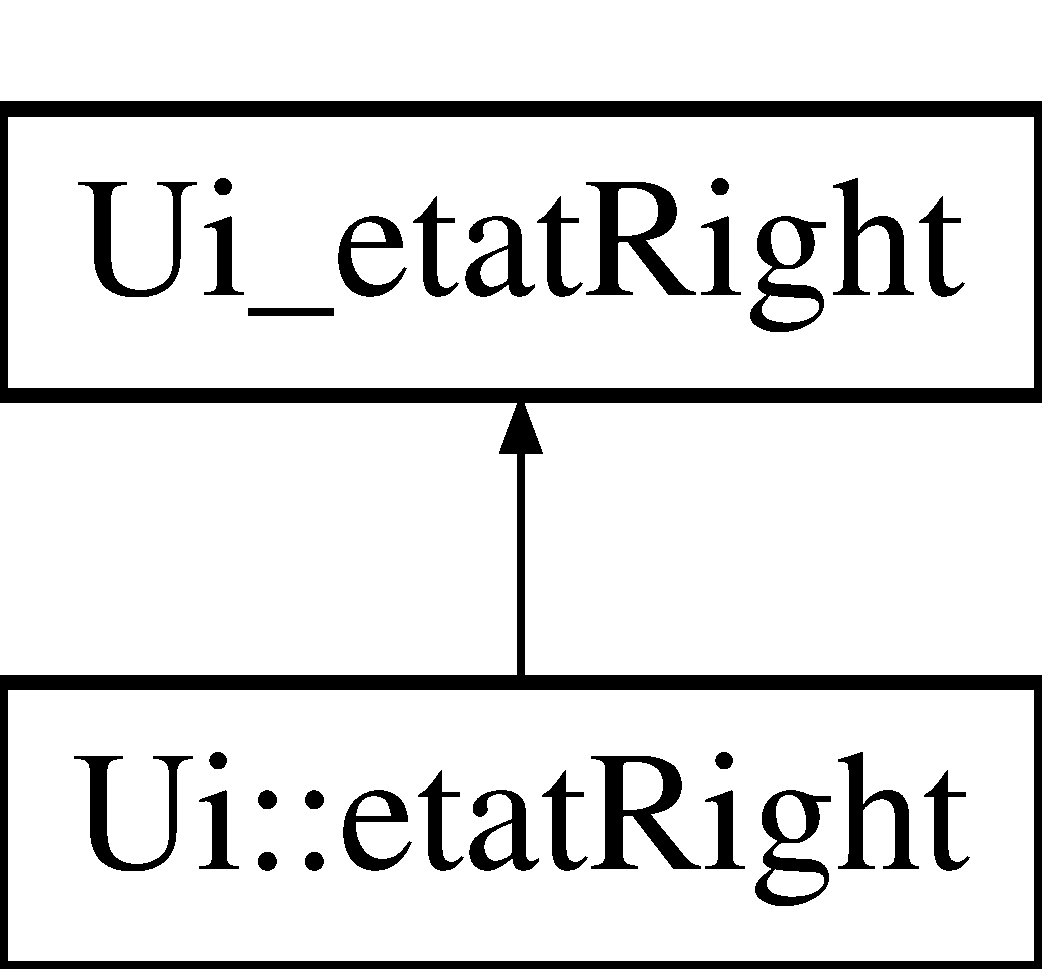
\includegraphics[height=2.000000cm]{class_ui_1_1etat_right}
\end{center}
\end{figure}
\subsection*{Additional Inherited Members}


The documentation for this class was generated from the following file\-:\begin{DoxyCompactItemize}
\item 
/home/aaiiighht/\-Bureau/projet\-T\-L/automate-\/project/ui\-\_\-etatright.\-h\end{DoxyCompactItemize}

\hypertarget{classetat_right}{\section{etat\-Right Class Reference}
\label{classetat_right}\index{etat\-Right@{etat\-Right}}
}
Inheritance diagram for etat\-Right\-:\begin{figure}[H]
\begin{center}
\leavevmode
\includegraphics[height=2.000000cm]{classetat_right}
\end{center}
\end{figure}
\subsection*{Public Slots}
\begin{DoxyCompactItemize}
\item 
void \hyperlink{classetat_right_a384a6718c6a76d7ad6c49ce8942e0f93}{add\-Transition} (int to, int vocab)
\begin{DoxyCompactList}\small\item\em Ajout d'une transition. \end{DoxyCompactList}\item 
void \hyperlink{classetat_right_a0ea39c8d918126244c9ecbf11b46a0ae}{erase\-Transition} (int to, int vocab)
\begin{DoxyCompactList}\small\item\em Suppresion d'une transition. \end{DoxyCompactList}\item 
\hypertarget{classetat_right_ac15456fc1dacf084b9bcbae7d6699627}{void {\bfseries etat\-Change} ()}\label{classetat_right_ac15456fc1dacf084b9bcbae7d6699627}

\end{DoxyCompactItemize}
\subsection*{Signals}
\begin{DoxyCompactItemize}
\item 
\hypertarget{classetat_right_ac7e6e4cff96fe796b6dcf1c4fca96e48}{void {\bfseries refresh\-Needed} (int)}\label{classetat_right_ac7e6e4cff96fe796b6dcf1c4fca96e48}

\item 
\hypertarget{classetat_right_a4ee395991e158ac64118b802d23b0962}{void {\bfseries etat\-Changes} (int, bool, bool)}\label{classetat_right_a4ee395991e158ac64118b802d23b0962}

\end{DoxyCompactItemize}
\subsection*{Public Member Functions}
\begin{DoxyCompactItemize}
\item 
\hyperlink{classetat_right_a9f171541e1762e55588f569a6c168dd3}{etat\-Right} (\hyperlink{class_automate}{Automate} $\ast$\hyperlink{classetat_right_aa6d344e0bd745915bfb4ea0e767f0bc0}{a}, int, Q\-Widget $\ast$parent=0)
\begin{DoxyCompactList}\small\item\em Constructeur. \end{DoxyCompactList}\item 
\hypertarget{classetat_right_a3e242d2baf785c43643f0bf9d8dec58f}{\hyperlink{classetat_right_a3e242d2baf785c43643f0bf9d8dec58f}{$\sim$etat\-Right} ()}\label{classetat_right_a3e242d2baf785c43643f0bf9d8dec58f}

\begin{DoxyCompactList}\small\item\em Destructeur. \end{DoxyCompactList}\item 
\hypertarget{classetat_right_a6631d8b4878cdaa7c8443c24825fd791}{void \hyperlink{classetat_right_a6631d8b4878cdaa7c8443c24825fd791}{remplir\-List\-Choix} ()}\label{classetat_right_a6631d8b4878cdaa7c8443c24825fd791}

\begin{DoxyCompactList}\small\item\em Remet à jour la liste dans \hyperlink{classchoix_pointe}{choix\-Pointe} permettant de choisir l'etat cible de la transition. \end{DoxyCompactList}\item 
\hypertarget{classetat_right_a9bd49810066fc43059d2adf138784fd6}{void {\bfseries add\-Visual\-Transition} (int, int)}\label{classetat_right_a9bd49810066fc43059d2adf138784fd6}

\item 
\hypertarget{classetat_right_a181683fbe813964220ddde7a048d840c}{void {\bfseries clean\-Trans} ()}\label{classetat_right_a181683fbe813964220ddde7a048d840c}

\end{DoxyCompactItemize}
\subsection*{Public Attributes}
\begin{DoxyCompactItemize}
\item 
\hyperlink{classchoix_pointe}{choix\-Pointe} $\ast$ \hyperlink{classetat_right_a1a3bbd118e907a6b9fe76ac22c702006}{add\-Trans}
\item 
\hyperlink{class_automate}{Automate} $\ast$ \hyperlink{classetat_right_aa6d344e0bd745915bfb4ea0e767f0bc0}{a}
\item 
int \hyperlink{classetat_right_ab061da0425585fa691f3766e3e81708c}{numero}
\end{DoxyCompactItemize}
\subsection*{Protected Member Functions}
\begin{DoxyCompactItemize}
\item 
\hypertarget{classetat_right_a0ca046ca45f51033a57401d90346dbec}{void {\bfseries change\-Event} (Q\-Event $\ast$e)}\label{classetat_right_a0ca046ca45f51033a57401d90346dbec}

\end{DoxyCompactItemize}


\subsection{Constructor \& Destructor Documentation}
\hypertarget{classetat_right_a9f171541e1762e55588f569a6c168dd3}{\index{etat\-Right@{etat\-Right}!etat\-Right@{etat\-Right}}
\index{etat\-Right@{etat\-Right}!etatRight@{etat\-Right}}
\subsubsection[{etat\-Right}]{\setlength{\rightskip}{0pt plus 5cm}etat\-Right\-::etat\-Right (
\begin{DoxyParamCaption}
\item[{{\bf Automate} $\ast$}]{a, }
\item[{int}]{number, }
\item[{Q\-Widget $\ast$}]{parent = {\ttfamily 0}}
\end{DoxyParamCaption}
)}}\label{classetat_right_a9f171541e1762e55588f569a6c168dd3}


Constructeur. 


\begin{DoxyParams}{Parameters}
{\em a} & \-: automate en cours de construction \\
\hline
\end{DoxyParams}


\subsection{Member Function Documentation}
\hypertarget{classetat_right_a384a6718c6a76d7ad6c49ce8942e0f93}{\index{etat\-Right@{etat\-Right}!add\-Transition@{add\-Transition}}
\index{add\-Transition@{add\-Transition}!etatRight@{etat\-Right}}
\subsubsection[{add\-Transition}]{\setlength{\rightskip}{0pt plus 5cm}void etat\-Right\-::add\-Transition (
\begin{DoxyParamCaption}
\item[{int}]{to, }
\item[{int}]{vocab}
\end{DoxyParamCaption}
)\hspace{0.3cm}{\ttfamily [slot]}}}\label{classetat_right_a384a6718c6a76d7ad6c49ce8942e0f93}


Ajout d'une transition. 


\begin{DoxyParams}{Parameters}
{\em to} & \-: numero de l'état cible \\
\hline
{\em vocab} & \-: etiquette de la transition \\
\hline
\end{DoxyParams}
\hypertarget{classetat_right_a0ea39c8d918126244c9ecbf11b46a0ae}{\index{etat\-Right@{etat\-Right}!erase\-Transition@{erase\-Transition}}
\index{erase\-Transition@{erase\-Transition}!etatRight@{etat\-Right}}
\subsubsection[{erase\-Transition}]{\setlength{\rightskip}{0pt plus 5cm}void etat\-Right\-::erase\-Transition (
\begin{DoxyParamCaption}
\item[{int}]{to, }
\item[{int}]{vocab}
\end{DoxyParamCaption}
)\hspace{0.3cm}{\ttfamily [slot]}}}\label{classetat_right_a0ea39c8d918126244c9ecbf11b46a0ae}


Suppresion d'une transition. 


\begin{DoxyParams}{Parameters}
{\em to} & \-: numero de l'état cible \\
\hline
{\em vocab} & \-: etiquette de la transition \\
\hline
\end{DoxyParams}


\subsection{Member Data Documentation}
\hypertarget{classetat_right_aa6d344e0bd745915bfb4ea0e767f0bc0}{\index{etat\-Right@{etat\-Right}!a@{a}}
\index{a@{a}!etatRight@{etat\-Right}}
\subsubsection[{a}]{\setlength{\rightskip}{0pt plus 5cm}{\bf Automate}$\ast$ etat\-Right\-::a}}\label{classetat_right_aa6d344e0bd745915bfb4ea0e767f0bc0}
Pointeur vers l'automate en construction \hypertarget{classetat_right_a1a3bbd118e907a6b9fe76ac22c702006}{\index{etat\-Right@{etat\-Right}!add\-Trans@{add\-Trans}}
\index{add\-Trans@{add\-Trans}!etatRight@{etat\-Right}}
\subsubsection[{add\-Trans}]{\setlength{\rightskip}{0pt plus 5cm}{\bf choix\-Pointe}$\ast$ etat\-Right\-::add\-Trans}}\label{classetat_right_a1a3bbd118e907a6b9fe76ac22c702006}
Pointeur vers l'objet \hyperlink{classchoix_pointe}{choix\-Pointe} permettant de gérer une transition \hypertarget{classetat_right_ab061da0425585fa691f3766e3e81708c}{\index{etat\-Right@{etat\-Right}!numero@{numero}}
\index{numero@{numero}!etatRight@{etat\-Right}}
\subsubsection[{numero}]{\setlength{\rightskip}{0pt plus 5cm}int etat\-Right\-::numero}}\label{classetat_right_ab061da0425585fa691f3766e3e81708c}
Numéro de l'état 

The documentation for this class was generated from the following files\-:\begin{DoxyCompactItemize}
\item 
/home/aaiiighht/\-Bureau/projet\-T\-L/automate-\/project/\hyperlink{etatright_8h}{etatright.\-h}\item 
/home/aaiiighht/\-Bureau/projet\-T\-L/automate-\/project/etatright.\-cpp\end{DoxyCompactItemize}

\input{class_ui_1_1_main_window}
\hypertarget{class_main_window}{\section{Main\-Window Class Reference}
\label{class_main_window}\index{Main\-Window@{Main\-Window}}
}


Inheritance diagram for Main\-Window\-:
\nopagebreak
\begin{figure}[H]
\begin{center}
\leavevmode
\includegraphics[width=160pt]{class_main_window__inherit__graph}
\end{center}
\end{figure}


Collaboration diagram for Main\-Window\-:
\nopagebreak
\begin{figure}[H]
\begin{center}
\leavevmode
\includegraphics[width=160pt]{class_main_window__coll__graph}
\end{center}
\end{figure}
\subsection*{Public Slots}
\begin{DoxyCompactItemize}
\item 
\hypertarget{class_main_window_a288b768c3c21a9171bdc56fe845ece8b}{void {\bfseries open\-File} ()}\label{class_main_window_a288b768c3c21a9171bdc56fe845ece8b}

\item 
\hypertarget{class_main_window_afc3b7768c20897733c1097fb5d956a6d}{void {\bfseries creer\-Auto} ()}\label{class_main_window_afc3b7768c20897733c1097fb5d956a6d}

\item 
\hypertarget{class_main_window_a2b49ea4a32d41b1a5a60c8d3b844a122}{void {\bfseries get\-Produit} ()}\label{class_main_window_a2b49ea4a32d41b1a5a60c8d3b844a122}

\item 
\hypertarget{class_main_window_ada476693941f6f33c5ec3c6089ec4058}{void {\bfseries get\-Determin} ()}\label{class_main_window_ada476693941f6f33c5ec3c6089ec4058}

\item 
\hypertarget{class_main_window_a5163f212156eecd4624ced33f1574361}{void {\bfseries get\-Suivant} ()}\label{class_main_window_a5163f212156eecd4624ced33f1574361}

\item 
\hypertarget{class_main_window_ad3f7fb432b87dd1c613d678cbc2b36fe}{void {\bfseries get\-Precedent} ()}\label{class_main_window_ad3f7fb432b87dd1c613d678cbc2b36fe}

\item 
\hypertarget{class_main_window_a8743d62b3db7581d930b2b8faa852ca7}{void {\bfseries get\-Standard} ()}\label{class_main_window_a8743d62b3db7581d930b2b8faa852ca7}

\item 
\hypertarget{class_main_window_ae0830e3c5a46ae29d7fd9cc870fe6c08}{void {\bfseries reset\-Ui} ()}\label{class_main_window_ae0830e3c5a46ae29d7fd9cc870fe6c08}

\item 
\hypertarget{class_main_window_adef6f7c5939e0e2b60414a55d716ddc8}{void {\bfseries test} ()}\label{class_main_window_adef6f7c5939e0e2b60414a55d716ddc8}

\item 
\hypertarget{class_main_window_a78f945084286506a64269d4ee75db224}{void {\bfseries info} ()}\label{class_main_window_a78f945084286506a64269d4ee75db224}

\end{DoxyCompactItemize}
\subsection*{Public Member Functions}
\begin{DoxyCompactItemize}
\item 
\hypertarget{class_main_window_a8b244be8b7b7db1b08de2a2acb9409db}{{\bfseries Main\-Window} (Q\-Widget $\ast$parent=0)}\label{class_main_window_a8b244be8b7b7db1b08de2a2acb9409db}

\item 
\hypertarget{class_main_window_a22ccaf0f029e895977c18774bf9ef115}{void {\bfseries start\-Layouting} ()}\label{class_main_window_a22ccaf0f029e895977c18774bf9ef115}

\item 
\hypertarget{class_main_window_ac9f5af352ce35293a2246f28af46b88c}{void {\bfseries affiche\-Automate} (\hyperlink{class_automate}{Automate})}\label{class_main_window_ac9f5af352ce35293a2246f28af46b88c}

\item 
\hypertarget{class_main_window_a7c730609e4e9f30d1b2dc88f8762a05c}{bool {\bfseries lire\-Dot} ()}\label{class_main_window_a7c730609e4e9f30d1b2dc88f8762a05c}

\item 
\hypertarget{class_main_window_ac9ec17b8cd9fe73a0cddfdc4423c9fb3}{bool {\bfseries lire\-Dot\-B} ()}\label{class_main_window_ac9ec17b8cd9fe73a0cddfdc4423c9fb3}

\end{DoxyCompactItemize}
\subsection*{Public Attributes}
\begin{DoxyCompactItemize}
\item 
\hypertarget{class_main_window_afe417a179b1efb0d372b4f8662cdd8e2}{Q\-Process $\ast$ {\bfseries Process\-T}}\label{class_main_window_afe417a179b1efb0d372b4f8662cdd8e2}

\item 
\hypertarget{class_main_window_a8edeaf68e7fac9c43d4b0cec2b859e90}{Q\-String {\bfseries program}}\label{class_main_window_a8edeaf68e7fac9c43d4b0cec2b859e90}

\end{DoxyCompactItemize}
\subsection*{Protected Member Functions}
\begin{DoxyCompactItemize}
\item 
\hypertarget{class_main_window_af4ca5d0d3d18ddcb7d54b6596bbf4797}{void {\bfseries change\-Event} (Q\-Event $\ast$e)}\label{class_main_window_af4ca5d0d3d18ddcb7d54b6596bbf4797}

\end{DoxyCompactItemize}


The documentation for this class was generated from the following files\-:\begin{DoxyCompactItemize}
\item 
/home/aaiiighht/\-Bureau/smartgit/bin/projet\-T\-L/automate-\/project/mainwindow.\-h\item 
/home/aaiiighht/\-Bureau/smartgit/bin/projet\-T\-L/automate-\/project/mainwindow.\-cpp\end{DoxyCompactItemize}

\hypertarget{structqt__meta__stringdata__choix_pointe__t}{\section{qt\-\_\-meta\-\_\-stringdata\-\_\-choix\-Pointe\-\_\-t Struct Reference}
\label{structqt__meta__stringdata__choix_pointe__t}\index{qt\-\_\-meta\-\_\-stringdata\-\_\-choix\-Pointe\-\_\-t@{qt\-\_\-meta\-\_\-stringdata\-\_\-choix\-Pointe\-\_\-t}}
}
\subsection*{Public Attributes}
\begin{DoxyCompactItemize}
\item 
\hypertarget{structqt__meta__stringdata__choix_pointe__t_ad3b353765e9d7e892b76492d283369d8}{Q\-Byte\-Array\-Data {\bfseries data} \mbox{[}6\mbox{]}}\label{structqt__meta__stringdata__choix_pointe__t_ad3b353765e9d7e892b76492d283369d8}

\item 
\hypertarget{structqt__meta__stringdata__choix_pointe__t_afc6132c465afb6133de2cea8933ef830}{char {\bfseries stringdata} \mbox{[}38\mbox{]}}\label{structqt__meta__stringdata__choix_pointe__t_afc6132c465afb6133de2cea8933ef830}

\end{DoxyCompactItemize}


The documentation for this struct was generated from the following file\-:\begin{DoxyCompactItemize}
\item 
/home/aaiiighht/\-Bureau/projet\-T\-L/automate-\/project/moc\-\_\-choixpointe.\-cpp\end{DoxyCompactItemize}

\hypertarget{structqt__meta__stringdata___create_automate__t}{\section{qt\-\_\-meta\-\_\-stringdata\-\_\-\-Create\-Automate\-\_\-t Struct Reference}
\label{structqt__meta__stringdata___create_automate__t}\index{qt\-\_\-meta\-\_\-stringdata\-\_\-\-Create\-Automate\-\_\-t@{qt\-\_\-meta\-\_\-stringdata\-\_\-\-Create\-Automate\-\_\-t}}
}
\subsection*{Public Attributes}
\begin{DoxyCompactItemize}
\item 
\hypertarget{structqt__meta__stringdata___create_automate__t_a210bd9798698d39b50889826c7b0cdc4}{Q\-Byte\-Array\-Data {\bfseries data} \mbox{[}11\mbox{]}}\label{structqt__meta__stringdata___create_automate__t_a210bd9798698d39b50889826c7b0cdc4}

\item 
\hypertarget{structqt__meta__stringdata___create_automate__t_ad815d5cc87bba2f46cb82e58f587d01c}{char {\bfseries stringdata} \mbox{[}114\mbox{]}}\label{structqt__meta__stringdata___create_automate__t_ad815d5cc87bba2f46cb82e58f587d01c}

\end{DoxyCompactItemize}


The documentation for this struct was generated from the following file\-:\begin{DoxyCompactItemize}
\item 
/home/aaiiighht/\-Bureau/smartgit/bin/projet\-T\-L/automate-\/project/moc\-\_\-createautomate.\-cpp\end{DoxyCompactItemize}

\hypertarget{structqt__meta__stringdata__etat_left__t}{\section{qt\-\_\-meta\-\_\-stringdata\-\_\-etat\-Left\-\_\-t Struct Reference}
\label{structqt__meta__stringdata__etat_left__t}\index{qt\-\_\-meta\-\_\-stringdata\-\_\-etat\-Left\-\_\-t@{qt\-\_\-meta\-\_\-stringdata\-\_\-etat\-Left\-\_\-t}}
}
\subsection*{Public Attributes}
\begin{DoxyCompactItemize}
\item 
\hypertarget{structqt__meta__stringdata__etat_left__t_ad16d3d553795be640d70bc3f777ad44c}{Q\-Byte\-Array\-Data {\bfseries data} \mbox{[}7\mbox{]}}\label{structqt__meta__stringdata__etat_left__t_ad16d3d553795be640d70bc3f777ad44c}

\item 
\hypertarget{structqt__meta__stringdata__etat_left__t_a091074801566ffe89515b5a1b998903e}{char {\bfseries stringdata} \mbox{[}53\mbox{]}}\label{structqt__meta__stringdata__etat_left__t_a091074801566ffe89515b5a1b998903e}

\end{DoxyCompactItemize}


The documentation for this struct was generated from the following file\-:\begin{DoxyCompactItemize}
\item 
/home/aaiiighht/\-Bureau/smartgit/bin/projet\-T\-L/automate-\/project/moc\-\_\-etatleft.\-cpp\end{DoxyCompactItemize}

\hypertarget{structqt__meta__stringdata__etat_right__t}{\section{qt\-\_\-meta\-\_\-stringdata\-\_\-etat\-Right\-\_\-t Struct Reference}
\label{structqt__meta__stringdata__etat_right__t}\index{qt\-\_\-meta\-\_\-stringdata\-\_\-etat\-Right\-\_\-t@{qt\-\_\-meta\-\_\-stringdata\-\_\-etat\-Right\-\_\-t}}
}
\subsection*{Public Attributes}
\begin{DoxyCompactItemize}
\item 
\hypertarget{structqt__meta__stringdata__etat_right__t_a23927212b2a8816af339c23e8667ee75}{Q\-Byte\-Array\-Data {\bfseries data} \mbox{[}7\mbox{]}}\label{structqt__meta__stringdata__etat_right__t_a23927212b2a8816af339c23e8667ee75}

\item 
\hypertarget{structqt__meta__stringdata__etat_right__t_a461a56b7dab2d4541ce1806226370f4e}{char {\bfseries stringdata} \mbox{[}79\mbox{]}}\label{structqt__meta__stringdata__etat_right__t_a461a56b7dab2d4541ce1806226370f4e}

\end{DoxyCompactItemize}


The documentation for this struct was generated from the following file\-:\begin{DoxyCompactItemize}
\item 
/home/aaiiighht/\-Bureau/smartgit/bin/projet\-T\-L/automate-\/project/moc\-\_\-etatright.\-cpp\end{DoxyCompactItemize}

\hypertarget{structqt__meta__stringdata___main_window__t}{\section{qt\-\_\-meta\-\_\-stringdata\-\_\-\-Main\-Window\-\_\-t Struct Reference}
\label{structqt__meta__stringdata___main_window__t}\index{qt\-\_\-meta\-\_\-stringdata\-\_\-\-Main\-Window\-\_\-t@{qt\-\_\-meta\-\_\-stringdata\-\_\-\-Main\-Window\-\_\-t}}
}
\subsection*{Public Attributes}
\begin{DoxyCompactItemize}
\item 
\hypertarget{structqt__meta__stringdata___main_window__t_a3425efb15419da867ddd69f8a4ed9e67}{Q\-Byte\-Array\-Data {\bfseries data} \mbox{[}13\mbox{]}}\label{structqt__meta__stringdata___main_window__t_a3425efb15419da867ddd69f8a4ed9e67}

\item 
\hypertarget{structqt__meta__stringdata___main_window__t_a83a4e6119d3600df5ed2ecd99c255853}{char {\bfseries stringdata} \mbox{[}125\mbox{]}}\label{structqt__meta__stringdata___main_window__t_a83a4e6119d3600df5ed2ecd99c255853}

\end{DoxyCompactItemize}


The documentation for this struct was generated from the following file\-:\begin{DoxyCompactItemize}
\item 
/home/aaiiighht/\-Bureau/projet\-T\-L/automate-\/project/moc\-\_\-mainwindow.\-cpp\end{DoxyCompactItemize}

\hypertarget{structqt__meta__stringdata___transition__t}{\section{qt\-\_\-meta\-\_\-stringdata\-\_\-\-Transition\-\_\-t Struct Reference}
\label{structqt__meta__stringdata___transition__t}\index{qt\-\_\-meta\-\_\-stringdata\-\_\-\-Transition\-\_\-t@{qt\-\_\-meta\-\_\-stringdata\-\_\-\-Transition\-\_\-t}}
}
\subsection*{Public Attributes}
\begin{DoxyCompactItemize}
\item 
\hypertarget{structqt__meta__stringdata___transition__t_a225b29f85eefacb8e10cfc21bdadc9c0}{Q\-Byte\-Array\-Data {\bfseries data} \mbox{[}4\mbox{]}}\label{structqt__meta__stringdata___transition__t_a225b29f85eefacb8e10cfc21bdadc9c0}

\item 
\hypertarget{structqt__meta__stringdata___transition__t_aead2c1958dd4a7dfd68b26587684a648}{char {\bfseries stringdata} \mbox{[}27\mbox{]}}\label{structqt__meta__stringdata___transition__t_aead2c1958dd4a7dfd68b26587684a648}

\end{DoxyCompactItemize}


The documentation for this struct was generated from the following file\-:\begin{DoxyCompactItemize}
\item 
/home/aaiiighht/\-Bureau/smartgit/bin/projet\-T\-L/automate-\/project/moc\-\_\-transition.\-cpp\end{DoxyCompactItemize}

\hypertarget{class_ui_1_1_transition}{\section{Ui\-:\-:Transition Class Reference}
\label{class_ui_1_1_transition}\index{Ui\-::\-Transition@{Ui\-::\-Transition}}
}
Inheritance diagram for Ui\-:\-:Transition\-:\begin{figure}[H]
\begin{center}
\leavevmode
\includegraphics[height=2.000000cm]{class_ui_1_1_transition}
\end{center}
\end{figure}
\subsection*{Additional Inherited Members}


The documentation for this class was generated from the following file\-:\begin{DoxyCompactItemize}
\item 
/home/aaiiighht/\-Bureau/projet\-T\-L/automate-\/project/ui\-\_\-transition.\-h\end{DoxyCompactItemize}

\hypertarget{class_transition}{\section{Transition Class Reference}
\label{class_transition}\index{Transition@{Transition}}
}
Inheritance diagram for Transition\-:\begin{figure}[H]
\begin{center}
\leavevmode
\includegraphics[height=2.000000cm]{class_transition}
\end{center}
\end{figure}
\subsection*{Public Slots}
\begin{DoxyCompactItemize}
\item 
\hypertarget{class_transition_a74d10ea64197661946db6d02b35b4cf1}{void \hyperlink{class_transition_a74d10ea64197661946db6d02b35b4cf1}{get\-Off} ()}\label{class_transition_a74d10ea64197661946db6d02b35b4cf1}

\begin{DoxyCompactList}\small\item\em Appelle la fonction eraser permettant de supprimer la transition. \end{DoxyCompactList}\end{DoxyCompactItemize}
\subsection*{Signals}
\begin{DoxyCompactItemize}
\item 
\hypertarget{class_transition_a926577e13d675e3caaf96660605e11a4}{void {\bfseries eraser} (int to, int \hyperlink{class_transition_a209c68fd432cd8e763342c1f2c784a87}{vocab})}\label{class_transition_a926577e13d675e3caaf96660605e11a4}

\end{DoxyCompactItemize}
\subsection*{Public Member Functions}
\begin{DoxyCompactItemize}
\item 
\hyperlink{class_transition_a3ac57c9b5df8a5a0247113611ba9d583}{Transition} (int to, int \hyperlink{class_transition_a209c68fd432cd8e763342c1f2c784a87}{vocab}, Q\-Widget $\ast$parent=0)
\begin{DoxyCompactList}\small\item\em Constructeur. \end{DoxyCompactList}\item 
\hyperlink{class_transition_ab66e8623f23c71cd4f07c69596427bab}{$\sim$\-Transition} ()
\begin{DoxyCompactList}\small\item\em Destructeur. \end{DoxyCompactList}\end{DoxyCompactItemize}
\subsection*{Public Attributes}
\begin{DoxyCompactItemize}
\item 
int \hyperlink{class_transition_a1b3f80305749c8f032a7f711527b0fc3}{cible}
\item 
int \hyperlink{class_transition_a209c68fd432cd8e763342c1f2c784a87}{vocab}
\end{DoxyCompactItemize}
\subsection*{Protected Member Functions}
\begin{DoxyCompactItemize}
\item 
\hypertarget{class_transition_a9df49098a20b28bd720e96d69255a026}{void {\bfseries change\-Event} (Q\-Event $\ast$e)}\label{class_transition_a9df49098a20b28bd720e96d69255a026}

\end{DoxyCompactItemize}


\subsection{Constructor \& Destructor Documentation}
\hypertarget{class_transition_a3ac57c9b5df8a5a0247113611ba9d583}{\index{Transition@{Transition}!Transition@{Transition}}
\index{Transition@{Transition}!Transition@{Transition}}
\subsubsection[{Transition}]{\setlength{\rightskip}{0pt plus 5cm}Transition\-::\-Transition (
\begin{DoxyParamCaption}
\item[{int}]{to, }
\item[{int}]{vocab, }
\item[{Q\-Widget $\ast$}]{parent = {\ttfamily 0}}
\end{DoxyParamCaption}
)}}\label{class_transition_a3ac57c9b5df8a5a0247113611ba9d583}


Constructeur. 

Construit la transition passée en paramètre


\begin{DoxyParams}{Parameters}
{\em to} & \-: numero de l'état cible de la transition \\
\hline
{\em vocab} & \-: etiquette de la transition \\
\hline
\end{DoxyParams}
\hypertarget{class_transition_ab66e8623f23c71cd4f07c69596427bab}{\index{Transition@{Transition}!$\sim$\-Transition@{$\sim$\-Transition}}
\index{$\sim$\-Transition@{$\sim$\-Transition}!Transition@{Transition}}
\subsubsection[{$\sim$\-Transition}]{\setlength{\rightskip}{0pt plus 5cm}Transition\-::$\sim$\-Transition (
\begin{DoxyParamCaption}
{}
\end{DoxyParamCaption}
)}}\label{class_transition_ab66e8623f23c71cd4f07c69596427bab}


Destructeur. 

Destructeur de la classe \hyperlink{class_transition}{Transition} 

\subsection{Member Data Documentation}
\hypertarget{class_transition_a1b3f80305749c8f032a7f711527b0fc3}{\index{Transition@{Transition}!cible@{cible}}
\index{cible@{cible}!Transition@{Transition}}
\subsubsection[{cible}]{\setlength{\rightskip}{0pt plus 5cm}int Transition\-::cible}}\label{class_transition_a1b3f80305749c8f032a7f711527b0fc3}
Numéro de l'état ciblé par la transition \hypertarget{class_transition_a209c68fd432cd8e763342c1f2c784a87}{\index{Transition@{Transition}!vocab@{vocab}}
\index{vocab@{vocab}!Transition@{Transition}}
\subsubsection[{vocab}]{\setlength{\rightskip}{0pt plus 5cm}int Transition\-::vocab}}\label{class_transition_a209c68fd432cd8e763342c1f2c784a87}
Numéro de l'étiquette portée par la transition 

The documentation for this class was generated from the following files\-:\begin{DoxyCompactItemize}
\item 
/home/aaiiighht/\-Bureau/projet\-T\-L/automate-\/project/\hyperlink{transition_8h}{transition.\-h}\item 
/home/aaiiighht/\-Bureau/projet\-T\-L/automate-\/project/transition.\-cpp\end{DoxyCompactItemize}

\hypertarget{class_ui__choix_pointe}{\section{Ui\-\_\-choix\-Pointe Class Reference}
\label{class_ui__choix_pointe}\index{Ui\-\_\-choix\-Pointe@{Ui\-\_\-choix\-Pointe}}
}
Inheritance diagram for Ui\-\_\-choix\-Pointe\-:\begin{figure}[H]
\begin{center}
\leavevmode
\includegraphics[height=2.000000cm]{class_ui__choix_pointe}
\end{center}
\end{figure}
\subsection*{Public Member Functions}
\begin{DoxyCompactItemize}
\item 
\hypertarget{class_ui__choix_pointe_afb01f288ce6a40c26c0346d1e0024f4e}{void {\bfseries setup\-Ui} (Q\-Widget $\ast$\hyperlink{classchoix_pointe}{choix\-Pointe})}\label{class_ui__choix_pointe_afb01f288ce6a40c26c0346d1e0024f4e}

\item 
\hypertarget{class_ui__choix_pointe_aea42cc3aeeb1ea76b18aeac75a7ec2cc}{void {\bfseries retranslate\-Ui} (Q\-Widget $\ast$\hyperlink{classchoix_pointe}{choix\-Pointe})}\label{class_ui__choix_pointe_aea42cc3aeeb1ea76b18aeac75a7ec2cc}

\end{DoxyCompactItemize}
\subsection*{Public Attributes}
\begin{DoxyCompactItemize}
\item 
\hypertarget{class_ui__choix_pointe_a226fc4022f79960aae1ebea672c9bc7d}{Q\-V\-Box\-Layout $\ast$ {\bfseries vertical\-Layout\-\_\-2}}\label{class_ui__choix_pointe_a226fc4022f79960aae1ebea672c9bc7d}

\item 
\hypertarget{class_ui__choix_pointe_ad66e9f3539981707ca70a32d850bec0c}{Q\-Frame $\ast$ {\bfseries Widget}}\label{class_ui__choix_pointe_ad66e9f3539981707ca70a32d850bec0c}

\item 
\hypertarget{class_ui__choix_pointe_ac9f65cb0e44cd91406847d94fa67137e}{Q\-H\-Box\-Layout $\ast$ {\bfseries horizontal\-Layout}}\label{class_ui__choix_pointe_ac9f65cb0e44cd91406847d94fa67137e}

\item 
\hypertarget{class_ui__choix_pointe_a5e603feb22929b35ea2822f8d4d013b5}{Q\-Label $\ast$ {\bfseries label\-\_\-3}}\label{class_ui__choix_pointe_a5e603feb22929b35ea2822f8d4d013b5}

\item 
\hypertarget{class_ui__choix_pointe_ae267664cffc2140c154a4137ecdf012d}{Q\-Combo\-Box $\ast$ {\bfseries les\-Choix}}\label{class_ui__choix_pointe_ae267664cffc2140c154a4137ecdf012d}

\item 
\hypertarget{class_ui__choix_pointe_a80c62d4b4e23a4727ac5e233f9dc8e59}{Q\-Label $\ast$ {\bfseries label\-\_\-4}}\label{class_ui__choix_pointe_a80c62d4b4e23a4727ac5e233f9dc8e59}

\item 
\hypertarget{class_ui__choix_pointe_a5cdc7c23b7939b46d87464ac59d6162a}{Q\-Line\-Edit $\ast$ {\bfseries line\-Edit}}\label{class_ui__choix_pointe_a5cdc7c23b7939b46d87464ac59d6162a}

\item 
\hypertarget{class_ui__choix_pointe_a762ac6f369982bd3e2972d88d7f92118}{Q\-Push\-Button $\ast$ {\bfseries push\-Button}}\label{class_ui__choix_pointe_a762ac6f369982bd3e2972d88d7f92118}

\end{DoxyCompactItemize}


The documentation for this class was generated from the following file\-:\begin{DoxyCompactItemize}
\item 
/home/aaiiighht/\-Bureau/projet\-T\-L/automate-\/project/ui\-\_\-choixpointe.\-h\end{DoxyCompactItemize}

\hypertarget{class_ui___create_automate}{\section{Ui\-\_\-\-Create\-Automate Class Reference}
\label{class_ui___create_automate}\index{Ui\-\_\-\-Create\-Automate@{Ui\-\_\-\-Create\-Automate}}
}


Inheritance diagram for Ui\-\_\-\-Create\-Automate\-:
\nopagebreak
\begin{figure}[H]
\begin{center}
\leavevmode
\includegraphics[width=184pt]{class_ui___create_automate__inherit__graph}
\end{center}
\end{figure}
\subsection*{Public Member Functions}
\begin{DoxyCompactItemize}
\item 
\hypertarget{class_ui___create_automate_adc1c604839808d7f0699c4c2075d119c}{void {\bfseries setup\-Ui} (Q\-Main\-Window $\ast$\hyperlink{class_create_automate}{Create\-Automate})}\label{class_ui___create_automate_adc1c604839808d7f0699c4c2075d119c}

\item 
\hypertarget{class_ui___create_automate_ac995057d86d1b7fd1f805ea116112e82}{void {\bfseries retranslate\-Ui} (Q\-Main\-Window $\ast$\hyperlink{class_create_automate}{Create\-Automate})}\label{class_ui___create_automate_ac995057d86d1b7fd1f805ea116112e82}

\item 
\hypertarget{class_ui___create_automate_adc1c604839808d7f0699c4c2075d119c}{void {\bfseries setup\-Ui} (Q\-Main\-Window $\ast$\hyperlink{class_create_automate}{Create\-Automate})}\label{class_ui___create_automate_adc1c604839808d7f0699c4c2075d119c}

\item 
\hypertarget{class_ui___create_automate_ac995057d86d1b7fd1f805ea116112e82}{void {\bfseries retranslate\-Ui} (Q\-Main\-Window $\ast$\hyperlink{class_create_automate}{Create\-Automate})}\label{class_ui___create_automate_ac995057d86d1b7fd1f805ea116112e82}

\end{DoxyCompactItemize}
\subsection*{Public Attributes}
\begin{DoxyCompactItemize}
\item 
\hypertarget{class_ui___create_automate_ab640344ed172ed3b3f99fc20dfca4ccd}{Q\-Action $\ast$ {\bfseries action\-Fermer}}\label{class_ui___create_automate_ab640344ed172ed3b3f99fc20dfca4ccd}

\item 
\hypertarget{class_ui___create_automate_a589a8428623e28a3099d25a54e6f5beb}{Q\-Action $\ast$ {\bfseries action\-Voir}}\label{class_ui___create_automate_a589a8428623e28a3099d25a54e6f5beb}

\item 
\hypertarget{class_ui___create_automate_a8f114b81317ce3fd1882aba860ebb1d5}{Q\-Action $\ast$ {\bfseries action\-Sauvegarder}}\label{class_ui___create_automate_a8f114b81317ce3fd1882aba860ebb1d5}

\item 
\hypertarget{class_ui___create_automate_a8e02ebfff985e61960f887a6bb5da12e}{Q\-Widget $\ast$ {\bfseries centralwidget}}\label{class_ui___create_automate_a8e02ebfff985e61960f887a6bb5da12e}

\item 
\hypertarget{class_ui___create_automate_ac82206485b1ada3e0c19f9e9b9efce03}{Q\-H\-Box\-Layout $\ast$ {\bfseries horizontal\-Layout}}\label{class_ui___create_automate_ac82206485b1ada3e0c19f9e9b9efce03}

\item 
\hypertarget{class_ui___create_automate_a193442b54e7ee51309918135f6dacc9f}{Q\-Frame $\ast$ {\bfseries frame}}\label{class_ui___create_automate_a193442b54e7ee51309918135f6dacc9f}

\item 
\hypertarget{class_ui___create_automate_a7d7e76f33c8d7e00bcb694e485d40a65}{Q\-V\-Box\-Layout $\ast$ {\bfseries etat\-Vert}}\label{class_ui___create_automate_a7d7e76f33c8d7e00bcb694e485d40a65}

\item 
\hypertarget{class_ui___create_automate_a1c4860add72420059ae41daf4920c993}{Q\-Push\-Button $\ast$ {\bfseries push\-Button}}\label{class_ui___create_automate_a1c4860add72420059ae41daf4920c993}

\item 
\hypertarget{class_ui___create_automate_aa9b0ea62072ad651d04b8149445cebab}{Q\-V\-Box\-Layout $\ast$ {\bfseries Droite}}\label{class_ui___create_automate_aa9b0ea62072ad651d04b8149445cebab}

\item 
\hypertarget{class_ui___create_automate_a68845d4a61e834e4b51ffdc0e4ba8ab6}{Q\-Frame $\ast$ {\bfseries frame1}}\label{class_ui___create_automate_a68845d4a61e834e4b51ffdc0e4ba8ab6}

\item 
\hypertarget{class_ui___create_automate_aff0664645be47986e5128f611ca67a89}{Q\-Grid\-Layout $\ast$ {\bfseries etat\-Droite}}\label{class_ui___create_automate_aff0664645be47986e5128f611ca67a89}

\item 
\hypertarget{class_ui___create_automate_a9824a119b2e2315f3431a8b2c8337f54}{Q\-Scroll\-Area $\ast$ {\bfseries scroll\-Area}}\label{class_ui___create_automate_a9824a119b2e2315f3431a8b2c8337f54}

\item 
\hypertarget{class_ui___create_automate_ac3a7890ea85d2b00cdca5284f03b752f}{Q\-Widget $\ast$ {\bfseries vue\-Tomate}}\label{class_ui___create_automate_ac3a7890ea85d2b00cdca5284f03b752f}

\item 
\hypertarget{class_ui___create_automate_a3fb88252da2468a423f9aee6b6244b6e}{Q\-Menu\-Bar $\ast$ {\bfseries menubar}}\label{class_ui___create_automate_a3fb88252da2468a423f9aee6b6244b6e}

\item 
\hypertarget{class_ui___create_automate_a391b79cdd9d7a9bd1e651c7efab7008f}{Q\-Menu $\ast$ {\bfseries menu\-Fichier}}\label{class_ui___create_automate_a391b79cdd9d7a9bd1e651c7efab7008f}

\item 
\hypertarget{class_ui___create_automate_a3067b908d77652d76719d3784443505e}{Q\-Tool\-Bar $\ast$ {\bfseries tool\-Bar}}\label{class_ui___create_automate_a3067b908d77652d76719d3784443505e}

\end{DoxyCompactItemize}


The documentation for this class was generated from the following file\-:\begin{DoxyCompactItemize}
\item 
/home/aaiiighht/\-Bureau/smartgit/bin/projet\-T\-L/automate-\/project/release/ui\-\_\-createautomate.\-h\end{DoxyCompactItemize}

\hypertarget{class_ui__etat_left}{\section{Ui\-\_\-etat\-Left Class Reference}
\label{class_ui__etat_left}\index{Ui\-\_\-etat\-Left@{Ui\-\_\-etat\-Left}}
}


Inheritance diagram for Ui\-\_\-etat\-Left\-:
\nopagebreak
\begin{figure}[H]
\begin{center}
\leavevmode
\includegraphics[width=144pt]{class_ui__etat_left__inherit__graph}
\end{center}
\end{figure}
\subsection*{Public Member Functions}
\begin{DoxyCompactItemize}
\item 
\hypertarget{class_ui__etat_left_a6ced76468569bc7b60f2f007c535091b}{void {\bfseries setup\-Ui} (Q\-Widget $\ast$\hyperlink{classetat_left}{etat\-Left})}\label{class_ui__etat_left_a6ced76468569bc7b60f2f007c535091b}

\item 
\hypertarget{class_ui__etat_left_a8a2d38afa659c1af5db423e286b41eda}{void {\bfseries retranslate\-Ui} (Q\-Widget $\ast$\hyperlink{classetat_left}{etat\-Left})}\label{class_ui__etat_left_a8a2d38afa659c1af5db423e286b41eda}

\item 
\hypertarget{class_ui__etat_left_a6ced76468569bc7b60f2f007c535091b}{void {\bfseries setup\-Ui} (Q\-Widget $\ast$\hyperlink{classetat_left}{etat\-Left})}\label{class_ui__etat_left_a6ced76468569bc7b60f2f007c535091b}

\item 
\hypertarget{class_ui__etat_left_a8a2d38afa659c1af5db423e286b41eda}{void {\bfseries retranslate\-Ui} (Q\-Widget $\ast$\hyperlink{classetat_left}{etat\-Left})}\label{class_ui__etat_left_a8a2d38afa659c1af5db423e286b41eda}

\end{DoxyCompactItemize}
\subsection*{Public Attributes}
\begin{DoxyCompactItemize}
\item 
\hypertarget{class_ui__etat_left_a274c9cd2b7f92638d78caf593154db32}{Q\-Grid\-Layout $\ast$ {\bfseries grid\-Layout}}\label{class_ui__etat_left_a274c9cd2b7f92638d78caf593154db32}

\item 
\hypertarget{class_ui__etat_left_adf0d56b2cf4c98e71862ab4e70b54745}{Q\-H\-Box\-Layout $\ast$ {\bfseries horizontal\-Layout}}\label{class_ui__etat_left_adf0d56b2cf4c98e71862ab4e70b54745}

\item 
\hypertarget{class_ui__etat_left_a0cabeb67430491c335b0a1638caa5231}{Q\-Spacer\-Item $\ast$ {\bfseries horizontal\-Spacer}}\label{class_ui__etat_left_a0cabeb67430491c335b0a1638caa5231}

\item 
\hypertarget{class_ui__etat_left_a596dbac3f6ee43e6e5ef5f469d9fd227}{Q\-Label $\ast$ {\bfseries label}}\label{class_ui__etat_left_a596dbac3f6ee43e6e5ef5f469d9fd227}

\item 
\hypertarget{class_ui__etat_left_a7122a5b8c6c69c99d33b250c507dfc50}{Q\-Spacer\-Item $\ast$ {\bfseries horizontal\-Spacer\-\_\-2}}\label{class_ui__etat_left_a7122a5b8c6c69c99d33b250c507dfc50}

\item 
\hypertarget{class_ui__etat_left_a7dc041bae70f473df0a8d2e564904191}{Q\-Push\-Button $\ast$ {\bfseries push\-Button}}\label{class_ui__etat_left_a7dc041bae70f473df0a8d2e564904191}

\item 
\hypertarget{class_ui__etat_left_a4c0c0bb1c5e29099a1154761ccb107e8}{Q\-Spacer\-Item $\ast$ {\bfseries horizontal\-Spacer\-\_\-3}}\label{class_ui__etat_left_a4c0c0bb1c5e29099a1154761ccb107e8}

\item 
\hypertarget{class_ui__etat_left_ab37a1ceedd6f15876f18720c51a3df43}{Q\-Push\-Button $\ast$ {\bfseries push\-Button\-\_\-2}}\label{class_ui__etat_left_ab37a1ceedd6f15876f18720c51a3df43}

\end{DoxyCompactItemize}


The documentation for this class was generated from the following file\-:\begin{DoxyCompactItemize}
\item 
/home/aaiiighht/\-Bureau/smartgit/bin/projet\-T\-L/automate-\/project/release/ui\-\_\-etatleft.\-h\end{DoxyCompactItemize}

\hypertarget{class_ui__etat_right}{\section{Ui\-\_\-etat\-Right Class Reference}
\label{class_ui__etat_right}\index{Ui\-\_\-etat\-Right@{Ui\-\_\-etat\-Right}}
}
Inheritance diagram for Ui\-\_\-etat\-Right\-:\begin{figure}[H]
\begin{center}
\leavevmode
\includegraphics[height=2.000000cm]{class_ui__etat_right}
\end{center}
\end{figure}
\subsection*{Public Member Functions}
\begin{DoxyCompactItemize}
\item 
\hypertarget{class_ui__etat_right_a19c54fd43d646f353282bc374f4c1e8a}{void {\bfseries setup\-Ui} (Q\-Widget $\ast$\hyperlink{classetat_right}{etat\-Right})}\label{class_ui__etat_right_a19c54fd43d646f353282bc374f4c1e8a}

\item 
\hypertarget{class_ui__etat_right_ae20f3075c259ee0be56cd0af3111dca5}{void {\bfseries retranslate\-Ui} (Q\-Widget $\ast$\hyperlink{classetat_right}{etat\-Right})}\label{class_ui__etat_right_ae20f3075c259ee0be56cd0af3111dca5}

\end{DoxyCompactItemize}
\subsection*{Public Attributes}
\begin{DoxyCompactItemize}
\item 
\hypertarget{class_ui__etat_right_ab111761269a0c67cd08f2381a575d636}{Q\-H\-Box\-Layout $\ast$ {\bfseries horizontal\-Layout}}\label{class_ui__etat_right_ab111761269a0c67cd08f2381a575d636}

\item 
\hypertarget{class_ui__etat_right_ab4333e10288126061814b741ac05be4f}{Q\-V\-Box\-Layout $\ast$ {\bfseries vertical\-Layout}}\label{class_ui__etat_right_ab4333e10288126061814b741ac05be4f}

\item 
\hypertarget{class_ui__etat_right_a66ec15f46d545ed5253055bbe5627919}{Q\-H\-Box\-Layout $\ast$ {\bfseries horizontal\-Layout\-\_\-3}}\label{class_ui__etat_right_a66ec15f46d545ed5253055bbe5627919}

\item 
\hypertarget{class_ui__etat_right_a0d656669f8cddbef0b2a7a1329f4a172}{Q\-Spacer\-Item $\ast$ {\bfseries horizontal\-Spacer}}\label{class_ui__etat_right_a0d656669f8cddbef0b2a7a1329f4a172}

\item 
\hypertarget{class_ui__etat_right_a69154a9d4ec3d146e1afcc8da5562f56}{Q\-Label $\ast$ {\bfseries label}}\label{class_ui__etat_right_a69154a9d4ec3d146e1afcc8da5562f56}

\item 
\hypertarget{class_ui__etat_right_acae8e9100665f802d47e037d18e81e10}{Q\-Spacer\-Item $\ast$ {\bfseries horizontal\-Spacer\-\_\-2}}\label{class_ui__etat_right_acae8e9100665f802d47e037d18e81e10}

\item 
\hypertarget{class_ui__etat_right_a8ba482a507b484fefb0d7e1eca110643}{Q\-H\-Box\-Layout $\ast$ {\bfseries horizontal\-Layout\-\_\-2}}\label{class_ui__etat_right_a8ba482a507b484fefb0d7e1eca110643}

\item 
\hypertarget{class_ui__etat_right_a12cad950322992284d7a9961d3df0e71}{Q\-Spacer\-Item $\ast$ {\bfseries horizontal\-Spacer\-\_\-3}}\label{class_ui__etat_right_a12cad950322992284d7a9961d3df0e71}

\item 
\hypertarget{class_ui__etat_right_a1c5e9932944d0c9ba19de130f4319a76}{Q\-Check\-Box $\ast$ {\bfseries check\-Box\-\_\-2}}\label{class_ui__etat_right_a1c5e9932944d0c9ba19de130f4319a76}

\item 
\hypertarget{class_ui__etat_right_ac9820c9b342d98aeb7628006d3680f8d}{Q\-Check\-Box $\ast$ {\bfseries check\-Box}}\label{class_ui__etat_right_ac9820c9b342d98aeb7628006d3680f8d}

\item 
\hypertarget{class_ui__etat_right_a70927b9537c904c9b08375b7b16f602a}{Q\-Spacer\-Item $\ast$ {\bfseries horizontal\-Spacer\-\_\-4}}\label{class_ui__etat_right_a70927b9537c904c9b08375b7b16f602a}

\item 
\hypertarget{class_ui__etat_right_a84fbc71af2dbce7ba9c121d3c8efb806}{Q\-H\-Box\-Layout $\ast$ {\bfseries Choix}}\label{class_ui__etat_right_a84fbc71af2dbce7ba9c121d3c8efb806}

\item 
\hypertarget{class_ui__etat_right_a6b6dd7a6a049e9eb6d6fcd25b4075830}{Q\-Frame $\ast$ {\bfseries frame}}\label{class_ui__etat_right_a6b6dd7a6a049e9eb6d6fcd25b4075830}

\item 
\hypertarget{class_ui__etat_right_a676317a105e9b63305fef82b234bba36}{Q\-V\-Box\-Layout $\ast$ {\bfseries Show\-Choix}}\label{class_ui__etat_right_a676317a105e9b63305fef82b234bba36}

\end{DoxyCompactItemize}


The documentation for this class was generated from the following file\-:\begin{DoxyCompactItemize}
\item 
/home/aaiiighht/\-Bureau/projet\-T\-L/automate-\/project/ui\-\_\-etatright.\-h\end{DoxyCompactItemize}

\hypertarget{class_ui___main_window}{\section{Ui\-\_\-\-Main\-Window Class Reference}
\label{class_ui___main_window}\index{Ui\-\_\-\-Main\-Window@{Ui\-\_\-\-Main\-Window}}
}


Inheritance diagram for Ui\-\_\-\-Main\-Window\-:
\nopagebreak
\begin{figure}[H]
\begin{center}
\leavevmode
\includegraphics[width=168pt]{class_ui___main_window__inherit__graph}
\end{center}
\end{figure}
\subsection*{Public Member Functions}
\begin{DoxyCompactItemize}
\item 
\hypertarget{class_ui___main_window_acf4a0872c4c77d8f43a2ec66ed849b58}{void {\bfseries setup\-Ui} (Q\-Main\-Window $\ast$\hyperlink{class_main_window}{Main\-Window})}\label{class_ui___main_window_acf4a0872c4c77d8f43a2ec66ed849b58}

\item 
\hypertarget{class_ui___main_window_a097dd160c3534a204904cb374412c618}{void {\bfseries retranslate\-Ui} (Q\-Main\-Window $\ast$\hyperlink{class_main_window}{Main\-Window})}\label{class_ui___main_window_a097dd160c3534a204904cb374412c618}

\item 
\hypertarget{class_ui___main_window_acf4a0872c4c77d8f43a2ec66ed849b58}{void {\bfseries setup\-Ui} (Q\-Main\-Window $\ast$\hyperlink{class_main_window}{Main\-Window})}\label{class_ui___main_window_acf4a0872c4c77d8f43a2ec66ed849b58}

\item 
\hypertarget{class_ui___main_window_a097dd160c3534a204904cb374412c618}{void {\bfseries retranslate\-Ui} (Q\-Main\-Window $\ast$\hyperlink{class_main_window}{Main\-Window})}\label{class_ui___main_window_a097dd160c3534a204904cb374412c618}

\end{DoxyCompactItemize}
\subsection*{Public Attributes}
\begin{DoxyCompactItemize}
\item 
\hypertarget{class_ui___main_window_a1bd115c56f0564a3ca045c03dd897348}{Q\-Action $\ast$ {\bfseries action\-Fermer}}\label{class_ui___main_window_a1bd115c56f0564a3ca045c03dd897348}

\item 
\hypertarget{class_ui___main_window_acd90a15adecbeec393675d84ab765050}{Q\-Action $\ast$ {\bfseries action\-New}}\label{class_ui___main_window_acd90a15adecbeec393675d84ab765050}

\item 
\hypertarget{class_ui___main_window_abb596b626c9b16ac38d65b4476d2e870}{Q\-Action $\ast$ {\bfseries action\-Faire\-Produit}}\label{class_ui___main_window_abb596b626c9b16ac38d65b4476d2e870}

\item 
\hypertarget{class_ui___main_window_aa0cf8fa88b8cd5d1600318f88fd2ef11}{Q\-Action $\ast$ {\bfseries action\-Ouvrir}}\label{class_ui___main_window_aa0cf8fa88b8cd5d1600318f88fd2ef11}

\item 
\hypertarget{class_ui___main_window_ab16761ce3a6c8c22679c26fee871e907}{Q\-Action $\ast$ {\bfseries action\-Voir}}\label{class_ui___main_window_ab16761ce3a6c8c22679c26fee871e907}

\item 
\hypertarget{class_ui___main_window_af7ffbc836902e12532279ca6bd12380d}{Q\-Action $\ast$ {\bfseries action\-Test}}\label{class_ui___main_window_af7ffbc836902e12532279ca6bd12380d}

\item 
\hypertarget{class_ui___main_window_afaf47b345d7e2cd3fd3134a09989f596}{Q\-Action $\ast$ {\bfseries action\-Clean}}\label{class_ui___main_window_afaf47b345d7e2cd3fd3134a09989f596}

\item 
\hypertarget{class_ui___main_window_a7975d448d8323606b7baaed3834a64b7}{Q\-Action $\ast$ {\bfseries action\-Info}}\label{class_ui___main_window_a7975d448d8323606b7baaed3834a64b7}

\item 
\hypertarget{class_ui___main_window_a297f8d7c373b5c4aba6b3eb9eff5f162}{Q\-Action $\ast$ {\bfseries action\-Determiniser}}\label{class_ui___main_window_a297f8d7c373b5c4aba6b3eb9eff5f162}

\item 
\hypertarget{class_ui___main_window_a6600dd3bdd3d55e535659e4a4096ea48}{Q\-Widget $\ast$ {\bfseries central\-Widget}}\label{class_ui___main_window_a6600dd3bdd3d55e535659e4a4096ea48}

\item 
\hypertarget{class_ui___main_window_ae7104d878681f568e492c5bd0f653157}{Q\-H\-Box\-Layout $\ast$ {\bfseries horizontal\-Layout}}\label{class_ui___main_window_ae7104d878681f568e492c5bd0f653157}

\item 
\hypertarget{class_ui___main_window_a649287f742c9a33b8444116dccb1b72b}{Q\-V\-Box\-Layout $\ast$ {\bfseries vertical\-Layout}}\label{class_ui___main_window_a649287f742c9a33b8444116dccb1b72b}

\item 
\hypertarget{class_ui___main_window_aececee7b1425eae3927a7b1b50b8e7a1}{Q\-H\-Box\-Layout $\ast$ {\bfseries Top\-Layout}}\label{class_ui___main_window_aececee7b1425eae3927a7b1b50b8e7a1}

\item 
\hypertarget{class_ui___main_window_a06ede9d5616fa7ece2407834b06e63ca}{Q\-Push\-Button $\ast$ {\bfseries bouton\-Prec}}\label{class_ui___main_window_a06ede9d5616fa7ece2407834b06e63ca}

\item 
\hypertarget{class_ui___main_window_add50bdf7cf6e00763015ca18be11ba2f}{Q\-Push\-Button $\ast$ {\bfseries bouton\-Suiv}}\label{class_ui___main_window_add50bdf7cf6e00763015ca18be11ba2f}

\item 
\hypertarget{class_ui___main_window_abd5208a614b390ce66b754a1237b5fb6}{Q\-H\-Box\-Layout $\ast$ {\bfseries Middle\-Layout}}\label{class_ui___main_window_abd5208a614b390ce66b754a1237b5fb6}

\item 
\hypertarget{class_ui___main_window_a5897afab91b4b2c58fede0c31c7ebadf}{Q\-Scroll\-Area $\ast$ {\bfseries scroll\-Area\-\_\-3}}\label{class_ui___main_window_a5897afab91b4b2c58fede0c31c7ebadf}

\item 
\hypertarget{class_ui___main_window_abd5c4050c781e0ec15d17274c0b7fff0}{Q\-Widget $\ast$ {\bfseries vue1}}\label{class_ui___main_window_abd5c4050c781e0ec15d17274c0b7fff0}

\item 
\hypertarget{class_ui___main_window_ab09a090bf29c2e48a3370d49708f7254}{Q\-Scroll\-Area $\ast$ {\bfseries scroll\-Area\-\_\-2}}\label{class_ui___main_window_ab09a090bf29c2e48a3370d49708f7254}

\item 
\hypertarget{class_ui___main_window_adc8b81436897eb53d06cf5491f5d5e09}{Q\-Widget $\ast$ {\bfseries vue2}}\label{class_ui___main_window_adc8b81436897eb53d06cf5491f5d5e09}

\item 
\hypertarget{class_ui___main_window_ac89148d0a6b333eb74b3ef8a7408ce09}{Q\-H\-Box\-Layout $\ast$ {\bfseries Lower\-Layout}}\label{class_ui___main_window_ac89148d0a6b333eb74b3ef8a7408ce09}

\item 
\hypertarget{class_ui___main_window_a5f80e22900f6e658019f6c50cbffea81}{Q\-Scroll\-Area $\ast$ {\bfseries scroll\-Area}}\label{class_ui___main_window_a5f80e22900f6e658019f6c50cbffea81}

\item 
\hypertarget{class_ui___main_window_a568bb8d49bc030a72568d6f3737fd180}{Q\-Widget $\ast$ {\bfseries vue\-Tomate}}\label{class_ui___main_window_a568bb8d49bc030a72568d6f3737fd180}

\item 
\hypertarget{class_ui___main_window_aaaf53df148a855801161abb4290683a0}{Q\-Text\-Edit $\ast$ {\bfseries label}}\label{class_ui___main_window_aaaf53df148a855801161abb4290683a0}

\item 
\hypertarget{class_ui___main_window_a502a50d7dc22415f511336bdfb4318b9}{Q\-Menu\-Bar $\ast$ {\bfseries menu\-Bar}}\label{class_ui___main_window_a502a50d7dc22415f511336bdfb4318b9}

\item 
\hypertarget{class_ui___main_window_a7ab5b88372fc7887d782937113c0ebbb}{Q\-Menu $\ast$ {\bfseries menu\-Fichier}}\label{class_ui___main_window_a7ab5b88372fc7887d782937113c0ebbb}

\item 
\hypertarget{class_ui___main_window_a0984bccf02cc63fd5cd1810af9e37185}{Q\-Tool\-Bar $\ast$ {\bfseries tool\-Bar\-\_\-2}}\label{class_ui___main_window_a0984bccf02cc63fd5cd1810af9e37185}

\item 
\hypertarget{class_ui___main_window_afa919f3af6f2f526a70f1fa331f63724}{Q\-Status\-Bar $\ast$ {\bfseries status\-Bar}}\label{class_ui___main_window_afa919f3af6f2f526a70f1fa331f63724}

\item 
\hypertarget{class_ui___main_window_aaa9d9c6e15ff9d685f907e3d15bcb2ee}{Q\-Action $\ast$ {\bfseries action\-Standardiser}}\label{class_ui___main_window_aaa9d9c6e15ff9d685f907e3d15bcb2ee}

\end{DoxyCompactItemize}


The documentation for this class was generated from the following file\-:\begin{DoxyCompactItemize}
\item 
/home/aaiiighht/\-Bureau/smartgit/bin/projet\-T\-L/automate-\/project/release/ui\-\_\-mainwindow.\-h\end{DoxyCompactItemize}

\hypertarget{class_ui___transition}{\section{Ui\-\_\-\-Transition Class Reference}
\label{class_ui___transition}\index{Ui\-\_\-\-Transition@{Ui\-\_\-\-Transition}}
}
Inheritance diagram for Ui\-\_\-\-Transition\-:\begin{figure}[H]
\begin{center}
\leavevmode
\includegraphics[height=2.000000cm]{class_ui___transition}
\end{center}
\end{figure}
\subsection*{Public Member Functions}
\begin{DoxyCompactItemize}
\item 
\hypertarget{class_ui___transition_a06f0129cc1a15bc1c50b55447578b1c5}{void {\bfseries setup\-Ui} (Q\-Widget $\ast$\hyperlink{class_transition}{Transition})}\label{class_ui___transition_a06f0129cc1a15bc1c50b55447578b1c5}

\item 
\hypertarget{class_ui___transition_ad9e6b3650adf1487f6d51e7c5d340427}{void {\bfseries retranslate\-Ui} (Q\-Widget $\ast$\hyperlink{class_transition}{Transition})}\label{class_ui___transition_ad9e6b3650adf1487f6d51e7c5d340427}

\end{DoxyCompactItemize}
\subsection*{Public Attributes}
\begin{DoxyCompactItemize}
\item 
\hypertarget{class_ui___transition_a4635f8a22e46362c42b1cf06bcd9b1cb}{Q\-H\-Box\-Layout $\ast$ {\bfseries horizontal\-Layout}}\label{class_ui___transition_a4635f8a22e46362c42b1cf06bcd9b1cb}

\item 
\hypertarget{class_ui___transition_a409e71244dde25cd75d063acfc56c534}{Q\-Label $\ast$ {\bfseries label}}\label{class_ui___transition_a409e71244dde25cd75d063acfc56c534}

\item 
\hypertarget{class_ui___transition_a0277cdf754c92b30522232be1bd05969}{Q\-Spacer\-Item $\ast$ {\bfseries horizontal\-Spacer}}\label{class_ui___transition_a0277cdf754c92b30522232be1bd05969}

\item 
\hypertarget{class_ui___transition_ab06520280ed48b79ae0878c5061767c8}{Q\-Push\-Button $\ast$ {\bfseries supress}}\label{class_ui___transition_ab06520280ed48b79ae0878c5061767c8}

\end{DoxyCompactItemize}


The documentation for this class was generated from the following file\-:\begin{DoxyCompactItemize}
\item 
/home/aaiiighht/\-Bureau/projet\-T\-L/automate-\/project/ui\-\_\-transition.\-h\end{DoxyCompactItemize}

\chapter{File Documentation}
\hypertarget{automate_8h}{\section{/home/aaiiighht/\-Bureau/projet\-T\-L/automate-\/project/automate.h File Reference}
\label{automate_8h}\index{/home/aaiiighht/\-Bureau/projet\-T\-L/automate-\/project/automate.\-h@{/home/aaiiighht/\-Bureau/projet\-T\-L/automate-\/project/automate.\-h}}
}


Représente un automate, son seul attribut est un vector d'états.  


{\ttfamily \#include $<$vector$>$}\\*
{\ttfamily \#include $<$set$>$}\\*
{\ttfamily \#include $<$list$>$}\\*
{\ttfamily \#include $<$map$>$}\\*
{\ttfamily \#include $<$string$>$}\\*
{\ttfamily \#include $<$cstdio$>$}\\*
{\ttfamily \#include $<$iostream$>$}\\*
{\ttfamily \#include $<$algorithm$>$}\\*
{\ttfamily \#include \char`\"{}etat.\-h\char`\"{}}\\*
\subsection*{Classes}
\begin{DoxyCompactItemize}
\item 
class \hyperlink{class_automate}{Automate}
\end{DoxyCompactItemize}
\subsection*{Functions}
\begin{DoxyCompactItemize}
\item 
bool \hyperlink{automate_8h_a9896d1263155efd59efe2a14ef2a807f}{equal} (list$<$ \hyperlink{classetat}{etat} $>$ \&l1, list$<$ \hyperlink{classetat}{etat} $>$ \&l2)
\begin{DoxyCompactList}\small\item\em Test l'égalité entre deux listes d'états. \end{DoxyCompactList}\item 
bool \hyperlink{automate_8h_adad60237c4515bce78983c4510406f70}{is\-Final} (list$<$ \hyperlink{classetat}{etat} $>$ l)
\begin{DoxyCompactList}\small\item\em Test si une liste d'états a au moins un état final. \end{DoxyCompactList}\end{DoxyCompactItemize}


\subsection{Detailed Description}
Représente un automate, son seul attribut est un vector d'états. 

\subsection{Function Documentation}
\hypertarget{automate_8h_a9896d1263155efd59efe2a14ef2a807f}{\index{automate.\-h@{automate.\-h}!equal@{equal}}
\index{equal@{equal}!automate.h@{automate.\-h}}
\subsubsection[{equal}]{\setlength{\rightskip}{0pt plus 5cm}bool equal (
\begin{DoxyParamCaption}
\item[{list$<$ {\bf etat} $>$ \&}]{l1, }
\item[{list$<$ {\bf etat} $>$ \&}]{l2}
\end{DoxyParamCaption}
)}}\label{automate_8h_a9896d1263155efd59efe2a14ef2a807f}


Test l'égalité entre deux listes d'états. 

Test l'égalité entre deux listes d'états l1 et l2

\begin{DoxyReturn}{Returns}
true si les listes sont égales, false sinon 
\end{DoxyReturn}
\hypertarget{automate_8h_adad60237c4515bce78983c4510406f70}{\index{automate.\-h@{automate.\-h}!is\-Final@{is\-Final}}
\index{is\-Final@{is\-Final}!automate.h@{automate.\-h}}
\subsubsection[{is\-Final}]{\setlength{\rightskip}{0pt plus 5cm}bool is\-Final (
\begin{DoxyParamCaption}
\item[{list$<$ {\bf etat} $>$}]{l}
\end{DoxyParamCaption}
)}}\label{automate_8h_adad60237c4515bce78983c4510406f70}


Test si une liste d'états a au moins un état final. 

Fonction utilisée seulement pour la déterminisation


\begin{DoxyParams}{Parameters}
{\em l} & \-: liste d'états testée\\
\hline
\end{DoxyParams}
\begin{DoxyReturn}{Returns}
true s'il y a au moins un état final dans la liste d'états, false sinon 
\end{DoxyReturn}

\hypertarget{mainwindow_8h}{\section{/home/aaiiighht/\-Bureau/projet\-T\-L/automate-\/project/mainwindow.h File Reference}
\label{mainwindow_8h}\index{/home/aaiiighht/\-Bureau/projet\-T\-L/automate-\/project/mainwindow.\-h@{/home/aaiiighht/\-Bureau/projet\-T\-L/automate-\/project/mainwindow.\-h}}
}


Représente la fenetre principale du programme. On gère ici les listeners des boutons.  


{\ttfamily \#include $<$Q\-Svg\-Widget$>$}\\*
{\ttfamily \#include $<$Q\-Main\-Window$>$}\\*
{\ttfamily \#include $<$Q\-Process$>$}\\*
{\ttfamily \#include $<$vector$>$}\\*
{\ttfamily \#include \char`\"{}automate.\-h\char`\"{}}\\*
{\ttfamily \#include $<$Q\-Push\-Button$>$}\\*
{\ttfamily \#include $<$Q\-File\-Dialog$>$}\\*
{\ttfamily \#include $<$Q\-Text\-Browser$>$}\\*
{\ttfamily \#include $<$Q\-Scroll\-Bar$>$}\\*
\subsection*{Classes}
\begin{DoxyCompactItemize}
\item 
class \hyperlink{class_main_window}{Main\-Window}
\end{DoxyCompactItemize}


\subsection{Detailed Description}
Représente la fenetre principale du programme. On gère ici les listeners des boutons. 
%--- End generated contents ---

% Index
\newpage
\phantomsection
\addcontentsline{toc}{chapter}{Index}
\printindex

\end{document}
